% Options for packages loaded elsewhere
\PassOptionsToPackage{unicode}{hyperref}
\PassOptionsToPackage{hyphens}{url}
%
\documentclass[
  ignorenonframetext,
]{beamer}
\usepackage{pgfpages}
\setbeamertemplate{caption}[numbered]
\setbeamertemplate{caption label separator}{: }
\setbeamercolor{caption name}{fg=normal text.fg}
\beamertemplatenavigationsymbolsempty
% Prevent slide breaks in the middle of a paragraph
\widowpenalties 1 10000
\raggedbottom
\setbeamertemplate{part page}{
  \centering
  \begin{beamercolorbox}[sep=16pt,center]{part title}
    \usebeamerfont{part title}\insertpart\par
  \end{beamercolorbox}
}
\setbeamertemplate{section page}{
  \centering
  \begin{beamercolorbox}[sep=12pt,center]{part title}
    \usebeamerfont{section title}\insertsection\par
  \end{beamercolorbox}
}
\setbeamertemplate{subsection page}{
  \centering
  \begin{beamercolorbox}[sep=8pt,center]{part title}
    \usebeamerfont{subsection title}\insertsubsection\par
  \end{beamercolorbox}
}
\AtBeginPart{
  \frame{\partpage}
}
\AtBeginSection{
  \ifbibliography
  \else
    \frame{\sectionpage}
  \fi
}
\AtBeginSubsection{
  \frame{\subsectionpage}
}

\usepackage{amsmath,amssymb}
\usepackage{iftex}
\ifPDFTeX
  \usepackage[T1]{fontenc}
  \usepackage[utf8]{inputenc}
  \usepackage{textcomp} % provide euro and other symbols
\else % if luatex or xetex
  \usepackage{unicode-math}
  \defaultfontfeatures{Scale=MatchLowercase}
  \defaultfontfeatures[\rmfamily]{Ligatures=TeX,Scale=1}
\fi
\usepackage{lmodern}
\ifPDFTeX\else  
    % xetex/luatex font selection
\fi
% Use upquote if available, for straight quotes in verbatim environments
\IfFileExists{upquote.sty}{\usepackage{upquote}}{}
\IfFileExists{microtype.sty}{% use microtype if available
  \usepackage[]{microtype}
  \UseMicrotypeSet[protrusion]{basicmath} % disable protrusion for tt fonts
}{}
\makeatletter
\@ifundefined{KOMAClassName}{% if non-KOMA class
  \IfFileExists{parskip.sty}{%
    \usepackage{parskip}
  }{% else
    \setlength{\parindent}{0pt}
    \setlength{\parskip}{6pt plus 2pt minus 1pt}}
}{% if KOMA class
  \KOMAoptions{parskip=half}}
\makeatother
\usepackage{xcolor}
\newif\ifbibliography
\setlength{\emergencystretch}{3em} % prevent overfull lines
\setcounter{secnumdepth}{-\maxdimen} % remove section numbering

\usepackage{color}
\usepackage{fancyvrb}
\newcommand{\VerbBar}{|}
\newcommand{\VERB}{\Verb[commandchars=\\\{\}]}
\DefineVerbatimEnvironment{Highlighting}{Verbatim}{commandchars=\\\{\}}
% Add ',fontsize=\small' for more characters per line
\usepackage{framed}
\definecolor{shadecolor}{RGB}{241,243,245}
\newenvironment{Shaded}{\begin{snugshade}}{\end{snugshade}}
\newcommand{\AlertTok}[1]{\textcolor[rgb]{0.68,0.00,0.00}{#1}}
\newcommand{\AnnotationTok}[1]{\textcolor[rgb]{0.37,0.37,0.37}{#1}}
\newcommand{\AttributeTok}[1]{\textcolor[rgb]{0.40,0.45,0.13}{#1}}
\newcommand{\BaseNTok}[1]{\textcolor[rgb]{0.68,0.00,0.00}{#1}}
\newcommand{\BuiltInTok}[1]{\textcolor[rgb]{0.00,0.23,0.31}{#1}}
\newcommand{\CharTok}[1]{\textcolor[rgb]{0.13,0.47,0.30}{#1}}
\newcommand{\CommentTok}[1]{\textcolor[rgb]{0.37,0.37,0.37}{#1}}
\newcommand{\CommentVarTok}[1]{\textcolor[rgb]{0.37,0.37,0.37}{\textit{#1}}}
\newcommand{\ConstantTok}[1]{\textcolor[rgb]{0.56,0.35,0.01}{#1}}
\newcommand{\ControlFlowTok}[1]{\textcolor[rgb]{0.00,0.23,0.31}{#1}}
\newcommand{\DataTypeTok}[1]{\textcolor[rgb]{0.68,0.00,0.00}{#1}}
\newcommand{\DecValTok}[1]{\textcolor[rgb]{0.68,0.00,0.00}{#1}}
\newcommand{\DocumentationTok}[1]{\textcolor[rgb]{0.37,0.37,0.37}{\textit{#1}}}
\newcommand{\ErrorTok}[1]{\textcolor[rgb]{0.68,0.00,0.00}{#1}}
\newcommand{\ExtensionTok}[1]{\textcolor[rgb]{0.00,0.23,0.31}{#1}}
\newcommand{\FloatTok}[1]{\textcolor[rgb]{0.68,0.00,0.00}{#1}}
\newcommand{\FunctionTok}[1]{\textcolor[rgb]{0.28,0.35,0.67}{#1}}
\newcommand{\ImportTok}[1]{\textcolor[rgb]{0.00,0.46,0.62}{#1}}
\newcommand{\InformationTok}[1]{\textcolor[rgb]{0.37,0.37,0.37}{#1}}
\newcommand{\KeywordTok}[1]{\textcolor[rgb]{0.00,0.23,0.31}{#1}}
\newcommand{\NormalTok}[1]{\textcolor[rgb]{0.00,0.23,0.31}{#1}}
\newcommand{\OperatorTok}[1]{\textcolor[rgb]{0.37,0.37,0.37}{#1}}
\newcommand{\OtherTok}[1]{\textcolor[rgb]{0.00,0.23,0.31}{#1}}
\newcommand{\PreprocessorTok}[1]{\textcolor[rgb]{0.68,0.00,0.00}{#1}}
\newcommand{\RegionMarkerTok}[1]{\textcolor[rgb]{0.00,0.23,0.31}{#1}}
\newcommand{\SpecialCharTok}[1]{\textcolor[rgb]{0.37,0.37,0.37}{#1}}
\newcommand{\SpecialStringTok}[1]{\textcolor[rgb]{0.13,0.47,0.30}{#1}}
\newcommand{\StringTok}[1]{\textcolor[rgb]{0.13,0.47,0.30}{#1}}
\newcommand{\VariableTok}[1]{\textcolor[rgb]{0.07,0.07,0.07}{#1}}
\newcommand{\VerbatimStringTok}[1]{\textcolor[rgb]{0.13,0.47,0.30}{#1}}
\newcommand{\WarningTok}[1]{\textcolor[rgb]{0.37,0.37,0.37}{\textit{#1}}}

\providecommand{\tightlist}{%
  \setlength{\itemsep}{0pt}\setlength{\parskip}{0pt}}\usepackage{longtable,booktabs,array}
\usepackage{calc} % for calculating minipage widths
\usepackage{caption}
% Make caption package work with longtable
\makeatletter
\def\fnum@table{\tablename~\thetable}
\makeatother
\usepackage{graphicx}
\makeatletter
\def\maxwidth{\ifdim\Gin@nat@width>\linewidth\linewidth\else\Gin@nat@width\fi}
\def\maxheight{\ifdim\Gin@nat@height>\textheight\textheight\else\Gin@nat@height\fi}
\makeatother
% Scale images if necessary, so that they will not overflow the page
% margins by default, and it is still possible to overwrite the defaults
% using explicit options in \includegraphics[width, height, ...]{}
\setkeys{Gin}{width=\maxwidth,height=\maxheight,keepaspectratio}
% Set default figure placement to htbp
\makeatletter
\def\fps@figure{htbp}
\makeatother

\makeatletter
\makeatother
\makeatletter
\makeatother
\makeatletter
\@ifpackageloaded{caption}{}{\usepackage{caption}}
\AtBeginDocument{%
\ifdefined\contentsname
  \renewcommand*\contentsname{Table of contents}
\else
  \newcommand\contentsname{Table of contents}
\fi
\ifdefined\listfigurename
  \renewcommand*\listfigurename{List of Figures}
\else
  \newcommand\listfigurename{List of Figures}
\fi
\ifdefined\listtablename
  \renewcommand*\listtablename{List of Tables}
\else
  \newcommand\listtablename{List of Tables}
\fi
\ifdefined\figurename
  \renewcommand*\figurename{Figure}
\else
  \newcommand\figurename{Figure}
\fi
\ifdefined\tablename
  \renewcommand*\tablename{Table}
\else
  \newcommand\tablename{Table}
\fi
}
\@ifpackageloaded{float}{}{\usepackage{float}}
\floatstyle{ruled}
\@ifundefined{c@chapter}{\newfloat{codelisting}{h}{lop}}{\newfloat{codelisting}{h}{lop}[chapter]}
\floatname{codelisting}{Listing}
\newcommand*\listoflistings{\listof{codelisting}{List of Listings}}
\makeatother
\makeatletter
\@ifpackageloaded{caption}{}{\usepackage{caption}}
\@ifpackageloaded{subcaption}{}{\usepackage{subcaption}}
\makeatother
\makeatletter
\@ifpackageloaded{tcolorbox}{}{\usepackage[skins,breakable]{tcolorbox}}
\makeatother
\makeatletter
\@ifundefined{shadecolor}{\definecolor{shadecolor}{rgb}{.97, .97, .97}}
\makeatother
\makeatletter
\makeatother
\makeatletter
\makeatother
\ifLuaTeX
  \usepackage{selnolig}  % disable illegal ligatures
\fi
\IfFileExists{bookmark.sty}{\usepackage{bookmark}}{\usepackage{hyperref}}
\IfFileExists{xurl.sty}{\usepackage{xurl}}{} % add URL line breaks if available
\urlstyle{same} % disable monospaced font for URLs
\hypersetup{
  pdftitle={Analysis of variance revisited},
  hidelinks,
  pdfcreator={LaTeX via pandoc}}

\title{Analysis of variance revisited}
\author{}
\date{}

\begin{document}
\frame{\titlepage}
\ifdefined\Shaded\renewenvironment{Shaded}{\begin{tcolorbox}[breakable, enhanced, boxrule=0pt, sharp corners, interior hidden, frame hidden, borderline west={3pt}{0pt}{shadecolor}]}{\end{tcolorbox}}\fi

\begin{frame}{Analysis of variance}
\protect\hypertarget{analysis-of-variance}{}
\begin{itemize}
\item
  Analysis of variance used with:

  \begin{itemize}
  \item
    counted/measured response
  \item
    categorical explanatory variable(s)
  \item
    that is, data divided into groups, and see if response significantly
    different among groups
  \item
    or, see whether knowing group membership helps to predict response.
  \end{itemize}
\end{itemize}
\end{frame}

\begin{frame}{Two stages}
\protect\hypertarget{two-stages}{}
\begin{itemize}
\item
  Typically two stages:

  \begin{itemize}
  \item
    \(F\)-test to detect \emph{any} differences among/due to groups
  \item
    if \(F\)-test significant, do \emph{multiple comparisons} to see
    which groups significantly different from which.
  \end{itemize}
\item
  Need special multiple comparisons method because just doing (say)
  two-sample \(t\)-tests on each pair of groups gives too big a chance
  of finding ``significant'' differences by accident.
\end{itemize}
\end{frame}

\begin{frame}[fragile]{Packages}
\protect\hypertarget{packages}{}
These:

\begin{Shaded}
\begin{Highlighting}[]
\FunctionTok{library}\NormalTok{(tidyverse)}
\FunctionTok{library}\NormalTok{(broom)}
\FunctionTok{library}\NormalTok{(car) }\CommentTok{\# for Levene\textquotesingle{}s text}
\end{Highlighting}
\end{Shaded}
\end{frame}

\begin{frame}{Example: Pain threshold and hair colour}
\protect\hypertarget{example-pain-threshold-and-hair-colour}{}
\begin{itemize}
\item
  Do people with different hair colour have different abilities to deal
  with pain?
\item
  Men and women of various ages divided into 4 groups by hair colour:
  light and dark blond, light and dark brown.
\item
  Each subject given a pain sensitivity test resulting in pain threshold
  score: higher score is higher pain tolerance.
\item
  19 subjects altogether.
\end{itemize}
\end{frame}

\begin{frame}[fragile]{The data}
\protect\hypertarget{the-data}{}
In \texttt{hairpain.txt}:

\begin{columns}[T]
\begin{column}{0.5\textwidth}
\begin{verbatim}
hair pain
lightblond 62
lightblond 60
lightblond 71
lightblond 55
lightblond 48
darkblond 63
darkblond 57
darkblond 52
darkblond 41
darkblond 43
\end{verbatim}
\end{column}

\begin{column}{5 0%\textwidth}
\begin{verbatim}
lightbrown 42
lightbrown 50
lightbrown 41
lightbrown 37
darkbrown 32
darkbrown 39
darkbrown 51
darkbrown 30
darkbrown 35
\end{verbatim}
\end{column}
\end{columns}
\end{frame}

\begin{frame}[fragile]{Summarizing the groups}
\protect\hypertarget{summarizing-the-groups}{}
\footnotesize

\begin{Shaded}
\begin{Highlighting}[]
\NormalTok{my\_url }\OtherTok{\textless{}{-}} \StringTok{"http://ritsokiguess.site/datafiles/hairpain.txt"}
\NormalTok{hairpain }\OtherTok{\textless{}{-}} \FunctionTok{read\_delim}\NormalTok{(my\_url, }\StringTok{" "}\NormalTok{)}
\NormalTok{hairpain }\SpecialCharTok{\%\textgreater{}\%}
  \FunctionTok{group\_by}\NormalTok{(hair) }\SpecialCharTok{\%\textgreater{}\%}
  \FunctionTok{summarize}\NormalTok{(}
    \AttributeTok{n =} \FunctionTok{n}\NormalTok{(),}
    \AttributeTok{xbar =} \FunctionTok{mean}\NormalTok{(pain),}
    \AttributeTok{s =} \FunctionTok{sd}\NormalTok{(pain)}
\NormalTok{  )}
\end{Highlighting}
\end{Shaded}

\begin{verbatim}
# A tibble: 4 x 4
  hair           n  xbar     s
  <chr>      <int> <dbl> <dbl>
1 darkblond      5  51.2  9.28
2 darkbrown      5  37.4  8.32
3 lightblond     5  59.2  8.53
4 lightbrown     4  42.5  5.45
\end{verbatim}

\normalsize

Brown-haired people seem to have lower pain tolerance.
\end{frame}

\begin{frame}[fragile]{Boxplot}
\protect\hypertarget{boxplot}{}
\begin{Shaded}
\begin{Highlighting}[]
\FunctionTok{ggplot}\NormalTok{(hairpain, }\FunctionTok{aes}\NormalTok{(}\AttributeTok{x =}\NormalTok{ hair, }\AttributeTok{y =}\NormalTok{ pain)) }\SpecialCharTok{+} \FunctionTok{geom\_boxplot}\NormalTok{()}
\end{Highlighting}
\end{Shaded}

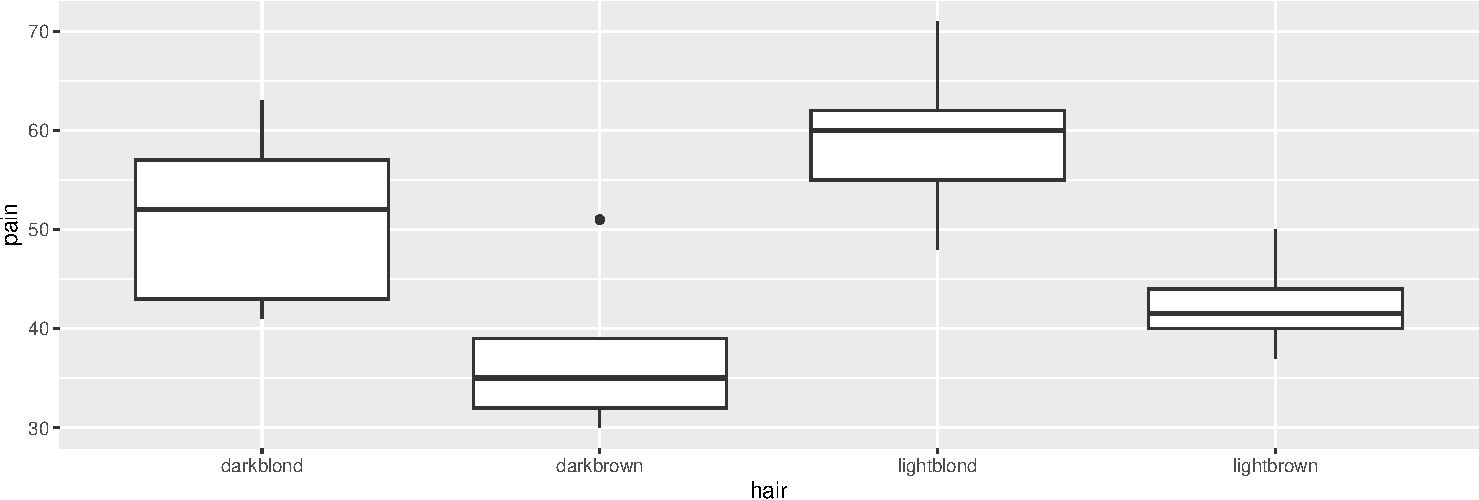
\includegraphics{anova_files/figure-beamer/tartuffo-1.pdf}
\end{frame}

\begin{frame}[fragile]{Assumptions}
\protect\hypertarget{assumptions}{}
\begin{itemize}
\item
  Data should be:

  \begin{itemize}
  \item
    normally distributed within each group
  \item
    same spread for each group
  \end{itemize}
\item
  \texttt{darkbrown} group has upper outlier (suggests not normal)
\item
  \texttt{darkblond} group has smaller IQR than other groups.
\item
  But, groups \emph{small}.
\item
  Shrug shoulders and continue for moment.
\end{itemize}
\end{frame}

\begin{frame}[fragile]{Testing equality of SDs}
\protect\hypertarget{testing-equality-of-sds}{}
\begin{itemize}
\tightlist
\item
  via \textbf{Levene's test} in package \texttt{car}:
\end{itemize}

\small

\begin{Shaded}
\begin{Highlighting}[]
\FunctionTok{leveneTest}\NormalTok{(pain }\SpecialCharTok{\textasciitilde{}}\NormalTok{ hair, }\AttributeTok{data =}\NormalTok{ hairpain)}
\end{Highlighting}
\end{Shaded}

\begin{verbatim}
Levene's Test for Homogeneity of Variance (center = median)
      Df F value Pr(>F)
group  3  0.3927   0.76
      15               
\end{verbatim}

\normalsize

\begin{itemize}
\item
  No evidence (at all) of difference among group SDs.
\item
  Possibly because groups \emph{small}.
\end{itemize}
\end{frame}

\begin{frame}[fragile]{Analysis of variance}
\protect\hypertarget{analysis-of-variance-1}{}
\small

\begin{Shaded}
\begin{Highlighting}[]
\NormalTok{hairpain}\FloatTok{.1} \OtherTok{\textless{}{-}} \FunctionTok{aov}\NormalTok{(pain }\SpecialCharTok{\textasciitilde{}}\NormalTok{ hair, }\AttributeTok{data =}\NormalTok{ hairpain)}
\FunctionTok{summary}\NormalTok{(hairpain}\FloatTok{.1}\NormalTok{)}
\end{Highlighting}
\end{Shaded}

\begin{verbatim}
            Df Sum Sq Mean Sq F value  Pr(>F)   
hair         3   1361   453.6   6.791 0.00411 **
Residuals   15   1002    66.8                   
---
Signif. codes:  0 '***' 0.001 '**' 0.01 '*' 0.05 '.' 0.1 ' ' 1
\end{verbatim}

\normalsize

\begin{itemize}
\item
  P-value small: the mean pain tolerances for the four groups are
  \emph{not} all the same.
\item
  Which groups differ from which, and how?
\end{itemize}
\end{frame}

\begin{frame}{Multiple comparisons}
\protect\hypertarget{multiple-comparisons}{}
\begin{itemize}
\item
  Which groups differ from which? Multiple comparisons method. Lots.
\item
  Problem: by comparing all the groups with each other, doing many
  tests, have large chance to (possibly incorrectly) reject \(H_0:\)
  groups have equal means.
\item
  4 groups: 6 comparisons (1 vs 2, 1 vs 3, \ldots, 3 vs 4). 5 groups: 10
  comparisons. Thus 6 (or 10) chances to make mistake.
\item
  Get ``familywise error rate'' of 0.05 (whatever), no matter how many
  comparisons you're doing.
\item
  My favourite: Tukey, or ``honestly significant differences'': how far
  apart might largest, smallest group means be (if actually no
  differences). Group means more different: significantly different.
\end{itemize}
\end{frame}

\begin{frame}[fragile]{Tukey}
\protect\hypertarget{tukey}{}
\begin{itemize}
\tightlist
\item
  \texttt{TukeyHSD:}
\end{itemize}

\footnotesize

\begin{Shaded}
\begin{Highlighting}[]
\FunctionTok{TukeyHSD}\NormalTok{(hairpain}\FloatTok{.1}\NormalTok{)}
\end{Highlighting}
\end{Shaded}

\begin{verbatim}
  Tukey multiple comparisons of means
    95% family-wise confidence level

Fit: aov(formula = pain ~ hair, data = hairpain)

$hair
                       diff        lwr        upr     p adj
darkbrown-darkblond   -13.8 -28.696741  1.0967407 0.0740679
lightblond-darkblond    8.0  -6.896741 22.8967407 0.4355768
lightbrown-darkblond   -8.7 -24.500380  7.1003795 0.4147283
lightblond-darkbrown   21.8   6.903259 36.6967407 0.0037079
lightbrown-darkbrown    5.1 -10.700380 20.9003795 0.7893211
lightbrown-lightblond -16.7 -32.500380 -0.8996205 0.0366467
\end{verbatim}

\normalsize
\end{frame}

\begin{frame}[fragile]{The old-fashioned way}
\protect\hypertarget{the-old-fashioned-way}{}
\begin{itemize}
\item
  List group means in order
\item
  Draw lines connecting groups that are \emph{not} significantly
  different:
\end{itemize}

\begin{verbatim}
darkbrown lightbrown  darkblond lightblond
37.4      42.5       51.2       59.2
-------------------------
                     ---------------
\end{verbatim}

\begin{itemize}
\item
  \texttt{lightblond} significantly higher than everything except
  \texttt{darkblond} (at \(\alpha=0.05\)).
\item
  \texttt{darkblond} in middle ground: not significantly less than
  \texttt{lightblond}, not significantly greater than \texttt{darkbrown}
  and \texttt{lightbrown}.
\item
  More data might resolve this.
\item
  Looks as if blond-haired people do have higher pain tolerance, but not
  completely clear.
\end{itemize}
\end{frame}

\begin{frame}{Some other multiple-comparison methods}
\protect\hypertarget{some-other-multiple-comparison-methods}{}
\begin{itemize}
\item
  Work any time you do \(k\) tests at once (not just ANOVA).

  \begin{itemize}
  \item
    \textbf{Bonferroni}: multiply all P-values by \(k\).
  \item
    \textbf{Holm}: multiply smallest P-value by \(k\), next-smallest by
    \(k-1\), etc.
  \item
    \textbf{False discovery rate}: multiply smallest P-value by \(k/1\),
    2nd-smallest by \(k/2\), \ldots, \(i\)-th smallest by \(k/i\).
  \end{itemize}
\item
  Stop after non-rejection.
\end{itemize}
\end{frame}

\begin{frame}{Example}
\protect\hypertarget{example}{}
\begin{itemize}
\item
  P-values 0.005, 0.015, 0.03, 0.06 (4 tests all done at once) Use
  \(\alpha=0.05\).
\item
  Bonferroni:

  \begin{itemize}
  \item
    Multiply all P-values by 4 (4 tests).
  \item
    Reject only 1st null.
  \end{itemize}
\item
  Holm:

  \begin{itemize}
  \item
    Times smallest P-value by 4: \(0.005*4=0.020<0.05\), reject.
  \item
    Times next smallest by 3: \(0.015*3=0.045<0.05\), reject.
  \item
    Times next smallest by 2: \(0.03*2=0.06>0.05\), do not reject. Stop.
  \end{itemize}
\end{itemize}
\end{frame}

\begin{frame}{\ldots Continued}
\protect\hypertarget{continued}{}
\begin{itemize}
\item
  With P-values 0.005, 0.015, 0.03, 0.06:
\item
  False discovery rate:

  \begin{itemize}
  \item
    Times smallest P-value by 4: \(0.005*4=0.02<0.05\): reject.
  \item
    Times second smallest by \(4/2\): \(0.015*4/2=0.03<0.05\), reject.
  \item
    Times third smallest by \(4/3\): \(0.03*4/3=0.04<0.05\), reject.
  \item
    Times fourth smallest by \(4/4\): \(0.06*4/4=0.06>0.05\), do not
    reject. Stop.
  \end{itemize}
\end{itemize}
\end{frame}

\begin{frame}[fragile]{\texttt{pairwise.t.test}}
\protect\hypertarget{pairwise.t.test}{}
\tiny

\begin{Shaded}
\begin{Highlighting}[]
\FunctionTok{with}\NormalTok{(hairpain, }\FunctionTok{pairwise.t.test}\NormalTok{(pain, hair, }\AttributeTok{p.adj =} \StringTok{"none"}\NormalTok{))}
\end{Highlighting}
\end{Shaded}

\begin{verbatim}

    Pairwise comparisons using t tests with pooled SD 

data:  pain and hair 

           darkblond darkbrown lightblond
darkbrown  0.01748   -         -         
lightblond 0.14251   0.00075   -         
lightbrown 0.13337   0.36695   0.00817   

P value adjustment method: none 
\end{verbatim}

\begin{Shaded}
\begin{Highlighting}[]
\FunctionTok{with}\NormalTok{(hairpain, }\FunctionTok{pairwise.t.test}\NormalTok{(pain, hair, }\AttributeTok{p.adj =} \StringTok{"holm"}\NormalTok{))}
\end{Highlighting}
\end{Shaded}

\begin{verbatim}

    Pairwise comparisons using t tests with pooled SD 

data:  pain and hair 

           darkblond darkbrown lightblond
darkbrown  0.0699    -         -         
lightblond 0.4001    0.0045    -         
lightbrown 0.4001    0.4001    0.0408    

P value adjustment method: holm 
\end{verbatim}

\normalsize
\end{frame}

\begin{frame}[fragile]{\texttt{pairwise.t.test} part 2}
\protect\hypertarget{pairwise.t.test-part-2}{}
\tiny

\begin{Shaded}
\begin{Highlighting}[]
\FunctionTok{with}\NormalTok{(hairpain, }\FunctionTok{pairwise.t.test}\NormalTok{(pain, hair, }\AttributeTok{p.adj =} \StringTok{"fdr"}\NormalTok{))}
\end{Highlighting}
\end{Shaded}

\begin{verbatim}

    Pairwise comparisons using t tests with pooled SD 

data:  pain and hair 

           darkblond darkbrown lightblond
darkbrown  0.0350    -         -         
lightblond 0.1710    0.0045    -         
lightbrown 0.1710    0.3670    0.0245    

P value adjustment method: fdr 
\end{verbatim}

\begin{Shaded}
\begin{Highlighting}[]
\FunctionTok{with}\NormalTok{(hairpain, }\FunctionTok{pairwise.t.test}\NormalTok{(pain, hair, }\AttributeTok{p.adj =} \StringTok{"bon"}\NormalTok{))}
\end{Highlighting}
\end{Shaded}

\begin{verbatim}

    Pairwise comparisons using t tests with pooled SD 

data:  pain and hair 

           darkblond darkbrown lightblond
darkbrown  0.1049    -         -         
lightblond 0.8550    0.0045    -         
lightbrown 0.8002    1.0000    0.0490    

P value adjustment method: bonferroni 
\end{verbatim}

\normalsize
\end{frame}

\begin{frame}{Comments}
\protect\hypertarget{comments}{}
\begin{itemize}
\item
  P-values all adjusted upwards from ``none''.
\item
  Required because 6 tests at once.
\item
  Highest P-values for Bonferroni: most ``conservative''.
\item
  Prefer Tukey or FDR or Holm.
\item
  Tukey only applies to ANOVA, not to other cases of multiple testing.
\end{itemize}
\end{frame}

\begin{frame}[fragile]{Rats and vitamin B}
\protect\hypertarget{rats-and-vitamin-b}{}
\begin{itemize}
\item
  What is the effect of dietary vitamin B on the kidney?
\item
  A number of rats were randomized to receive either a B-supplemented
  diet or a regular diet.
\item
  Desired to control for initial size of rats, so classified into size
  classes \texttt{lean} and \texttt{obese}.
\item
  After 20 weeks, rats' kidneys weighed.
\item
  Variables:

  \begin{itemize}
  \item
    Response: \texttt{kidneyweight} (grams).
  \item
    Explanatory: \texttt{diet}, \texttt{ratsize}.
  \end{itemize}
\item
  Read in data:
\end{itemize}

\small

\begin{Shaded}
\begin{Highlighting}[]
\NormalTok{my\_url }\OtherTok{\textless{}{-}} \StringTok{"http://ritsokiguess.site/datafiles/vitaminb.txt"}
\NormalTok{vitaminb }\OtherTok{\textless{}{-}} \FunctionTok{read\_delim}\NormalTok{(my\_url, }\StringTok{" "}\NormalTok{)}
\end{Highlighting}
\end{Shaded}

\normalsize
\end{frame}

\begin{frame}[fragile]{The data}
\protect\hypertarget{the-data-1}{}
\begin{Shaded}
\begin{Highlighting}[]
\NormalTok{vitaminb}
\end{Highlighting}
\end{Shaded}

\begin{verbatim}
# A tibble: 28 x 3
   ratsize diet     kidneyweight
   <chr>   <chr>           <dbl>
 1 lean    regular          1.62
 2 lean    regular          1.8 
 3 lean    regular          1.71
 4 lean    regular          1.81
 5 lean    regular          1.47
 6 lean    regular          1.37
 7 lean    regular          1.71
 8 lean    vitaminb         1.51
 9 lean    vitaminb         1.65
10 lean    vitaminb         1.45
# i 18 more rows
\end{verbatim}
\end{frame}

\begin{frame}[fragile]{Grouped boxplot}
\protect\hypertarget{grouped-boxplot}{}
\begin{Shaded}
\begin{Highlighting}[]
\FunctionTok{ggplot}\NormalTok{(vitaminb, }\FunctionTok{aes}\NormalTok{(}
  \AttributeTok{x =}\NormalTok{ ratsize, }\AttributeTok{y =}\NormalTok{ kidneyweight,}
  \AttributeTok{fill =}\NormalTok{ diet}
\NormalTok{)) }\SpecialCharTok{+} \FunctionTok{geom\_boxplot}\NormalTok{()}
\end{Highlighting}
\end{Shaded}

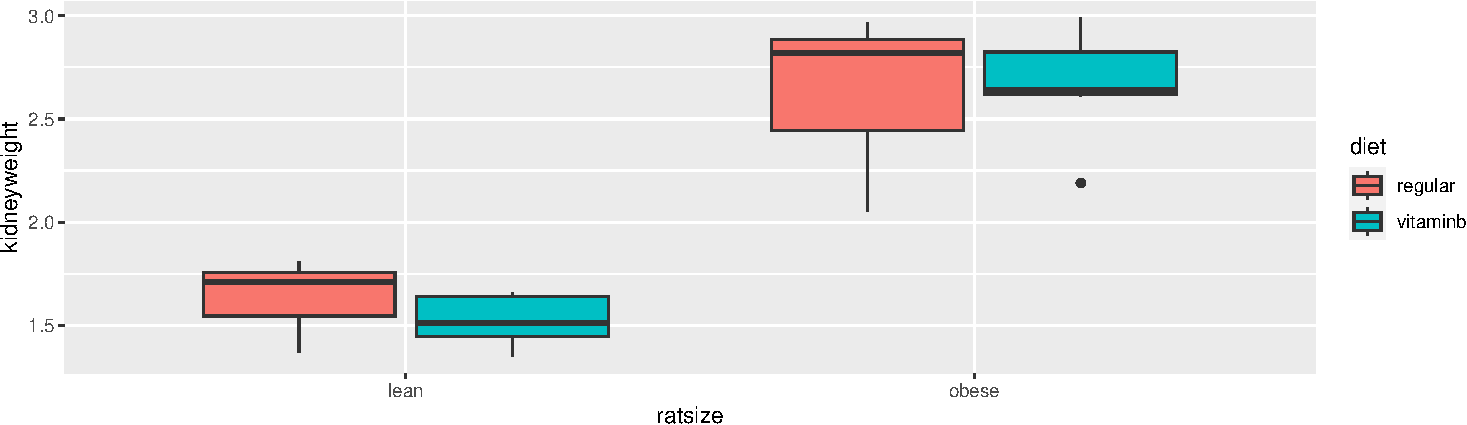
\includegraphics{anova_files/figure-beamer/bAnova-10-1.pdf}
\end{frame}

\begin{frame}[fragile]{What's going on?}
\protect\hypertarget{whats-going-on}{}
\begin{itemize}
\tightlist
\item
  Calculate group means:
\end{itemize}

\footnotesize

\begin{Shaded}
\begin{Highlighting}[]
\NormalTok{summary }\OtherTok{\textless{}{-}}\NormalTok{ vitaminb }\SpecialCharTok{\%\textgreater{}\%}
  \FunctionTok{group\_by}\NormalTok{(ratsize, diet) }\SpecialCharTok{\%\textgreater{}\%}
  \FunctionTok{summarize}\NormalTok{(}\AttributeTok{mean =} \FunctionTok{mean}\NormalTok{(kidneyweight))}
\NormalTok{summary}
\end{Highlighting}
\end{Shaded}

\begin{verbatim}
# A tibble: 4 x 3
# Groups:   ratsize [2]
  ratsize diet      mean
  <chr>   <chr>    <dbl>
1 lean    regular   1.64
2 lean    vitaminb  1.53
3 obese   regular   2.64
4 obese   vitaminb  2.67
\end{verbatim}

\normalsize

\begin{itemize}
\item
  Rat size: a large and consistent effect.
\item
  Diet: small/no effect (compare same rat size, different diet).
\item
  Effect of rat size \emph{same} for each diet: no interaction.
\end{itemize}
\end{frame}

\begin{frame}[fragile]{ANOVA with interaction}
\protect\hypertarget{anova-with-interaction}{}
\begin{Shaded}
\begin{Highlighting}[]
\NormalTok{vitaminb}\FloatTok{.1} \OtherTok{\textless{}{-}} \FunctionTok{aov}\NormalTok{(kidneyweight }\SpecialCharTok{\textasciitilde{}}\NormalTok{ ratsize }\SpecialCharTok{*}\NormalTok{ diet,}
  \AttributeTok{data =}\NormalTok{ vitaminb}
\NormalTok{)}
\FunctionTok{summary}\NormalTok{(vitaminb}\FloatTok{.1}\NormalTok{)}
\end{Highlighting}
\end{Shaded}

\begin{verbatim}
             Df Sum Sq Mean Sq F value   Pr(>F)    
ratsize       1  8.068   8.068 141.179 1.53e-11 ***
diet          1  0.012   0.012   0.218    0.645    
ratsize:diet  1  0.036   0.036   0.638    0.432    
Residuals    24  1.372   0.057                     
---
Signif. codes:  0 '***' 0.001 '**' 0.01 '*' 0.05 '.' 0.1 ' ' 1
\end{verbatim}

\begin{itemize}
\tightlist
\item
  Significance/nonsignificance as we expected.
\item
  Note no significant interaction (can be removed).
\end{itemize}
\end{frame}

\begin{frame}[fragile]{Interaction plot}
\protect\hypertarget{interaction-plot}{}
\begin{itemize}
\tightlist
\item
  Plot mean of response variable against one of the explanatory, using
  other one as groups. Start from \texttt{summary}:
\end{itemize}

\begin{Shaded}
\begin{Highlighting}[]
\NormalTok{g }\OtherTok{\textless{}{-}} \FunctionTok{ggplot}\NormalTok{(summary, }\FunctionTok{aes}\NormalTok{(}
  \AttributeTok{x =}\NormalTok{ ratsize, }\AttributeTok{y =}\NormalTok{ mean,}
  \AttributeTok{colour =}\NormalTok{ diet, }\AttributeTok{group =}\NormalTok{ diet}
\NormalTok{)) }\SpecialCharTok{+}
  \FunctionTok{geom\_point}\NormalTok{() }\SpecialCharTok{+} \FunctionTok{geom\_line}\NormalTok{()}
\end{Highlighting}
\end{Shaded}

\begin{itemize}
\tightlist
\item
  For this, have to give \emph{both} \texttt{group} and \texttt{colour}.
\end{itemize}
\end{frame}

\begin{frame}[fragile]{The interaction plot}
\protect\hypertarget{the-interaction-plot}{}
\begin{Shaded}
\begin{Highlighting}[]
\NormalTok{g}
\end{Highlighting}
\end{Shaded}

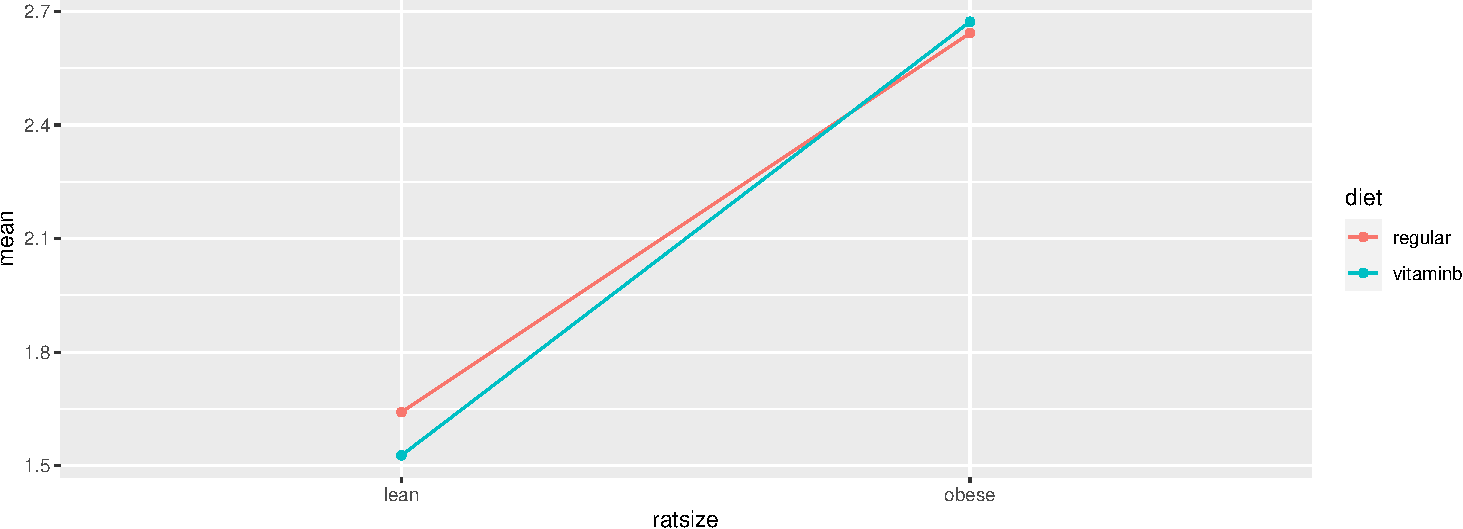
\includegraphics{anova_files/figure-beamer/bAnova-14-1.pdf}

Lines basically parallel, indicating no interaction.
\end{frame}

\begin{frame}[fragile]{Take out interaction}
\protect\hypertarget{take-out-interaction}{}
\small

\begin{Shaded}
\begin{Highlighting}[]
\NormalTok{vitaminb}\FloatTok{.2} \OtherTok{\textless{}{-}} \FunctionTok{update}\NormalTok{(vitaminb}\FloatTok{.1}\NormalTok{, . }\SpecialCharTok{\textasciitilde{}}\NormalTok{ . }\SpecialCharTok{{-}}\NormalTok{ ratsize}\SpecialCharTok{:}\NormalTok{diet)}
\FunctionTok{summary}\NormalTok{(vitaminb}\FloatTok{.2}\NormalTok{)}
\end{Highlighting}
\end{Shaded}

\begin{verbatim}
            Df Sum Sq Mean Sq F value   Pr(>F)    
ratsize      1  8.068   8.068 143.256 7.59e-12 ***
diet         1  0.012   0.012   0.221    0.643    
Residuals   25  1.408   0.056                     
---
Signif. codes:  0 '***' 0.001 '**' 0.01 '*' 0.05 '.' 0.1 ' ' 1
\end{verbatim}

\normalsize

\begin{itemize}
\item
  No Tukey for \texttt{diet}: not significant.
\item
  No Tukey for \texttt{ratsize}: only two sizes, and already know that
  obese rats have larger kidneys than lean ones.
\item
  Bottom line: diet has no effect on kidney size once you control for
  size of rat.
\end{itemize}
\end{frame}

\begin{frame}{Assessing assumptions: residuals}
\protect\hypertarget{assessing-assumptions-residuals}{}
\begin{itemize}
\tightlist
\item
  In two-way ANOVA, not many observations per treatment group.
\item
  Difficult to check for normality / equal spreads.
\item
  \emph{But}, any regular ANOVA also a regression.
\item
  Use regression residual ideas.
\item
  In ANOVA, one fitted value per treatment group (based on means).
\item
  Residual: observation minus fitted value.
\end{itemize}
\end{frame}

\begin{frame}[fragile]{Previous ANOVA as regression}
\protect\hypertarget{previous-anova-as-regression}{}
\scriptsize

\begin{Shaded}
\begin{Highlighting}[]
\NormalTok{vitaminb}\FloatTok{.3} \OtherTok{\textless{}{-}} \FunctionTok{lm}\NormalTok{(kidneyweight }\SpecialCharTok{\textasciitilde{}}\NormalTok{ ratsize }\SpecialCharTok{+}\NormalTok{ diet, }\AttributeTok{data =}\NormalTok{ vitaminb)}
\FunctionTok{summary}\NormalTok{(vitaminb}\FloatTok{.3}\NormalTok{)}
\end{Highlighting}
\end{Shaded}

\begin{verbatim}

Call:
lm(formula = kidneyweight ~ ratsize + diet, data = vitaminb)

Residuals:
     Min       1Q   Median       3Q      Max 
-0.62893 -0.12625  0.04071  0.14607  0.35321 

Coefficients:
             Estimate Std. Error t value Pr(>|t|)    
(Intercept)   1.60536    0.07768   20.67  < 2e-16 ***
ratsizeobese  1.07357    0.08970   11.97 7.59e-12 ***
dietvitaminb -0.04214    0.08970   -0.47    0.643    
---
Signif. codes:  0 '***' 0.001 '**' 0.01 '*' 0.05 '.' 0.1 ' ' 1

Residual standard error: 0.2373 on 25 degrees of freedom
Multiple R-squared:  0.8516,    Adjusted R-squared:  0.8397 
F-statistic: 71.74 on 2 and 25 DF,  p-value: 4.39e-11
\end{verbatim}

\normalsize
\end{frame}

\begin{frame}[fragile]{Reproduce ANOVA}
\protect\hypertarget{reproduce-anova}{}
\small

\begin{Shaded}
\begin{Highlighting}[]
  \FunctionTok{drop1}\NormalTok{(vitaminb}\FloatTok{.3}\NormalTok{, }\AttributeTok{test =} \StringTok{"F"}\NormalTok{) }
\end{Highlighting}
\end{Shaded}

\begin{verbatim}
Single term deletions

Model:
kidneyweight ~ ratsize + diet
        Df Sum of Sq    RSS     AIC  F value    Pr(>F)    
<none>               1.4079 -77.722                       
ratsize  1    8.0679 9.4758 -26.337 143.2563 7.593e-12 ***
diet     1    0.0124 1.4204 -79.476   0.2207    0.6425    
---
Signif. codes:  0 '***' 0.001 '**' 0.01 '*' 0.05 '.' 0.1 ' ' 1
\end{verbatim}

\normalsize

\begin{itemize}
\tightlist
\item
  ANOVA and regression \texttt{drop1} output always the same.
\item
  this time, ANOVA and regression \texttt{summary} output have same
  P-values, but only because categorical variables both have two levels.
\end{itemize}
\end{frame}

\begin{frame}[fragile]{Are the residuals normal?}
\protect\hypertarget{are-the-residuals-normal}{}
\begin{Shaded}
\begin{Highlighting}[]
\FunctionTok{ggplot}\NormalTok{(vitaminb}\FloatTok{.3}\NormalTok{, }\FunctionTok{aes}\NormalTok{(}\AttributeTok{sample=}\NormalTok{.resid)) }\SpecialCharTok{+} 
  \FunctionTok{stat\_qq}\NormalTok{() }\SpecialCharTok{+} \FunctionTok{stat\_qq\_line}\NormalTok{()}
\end{Highlighting}
\end{Shaded}

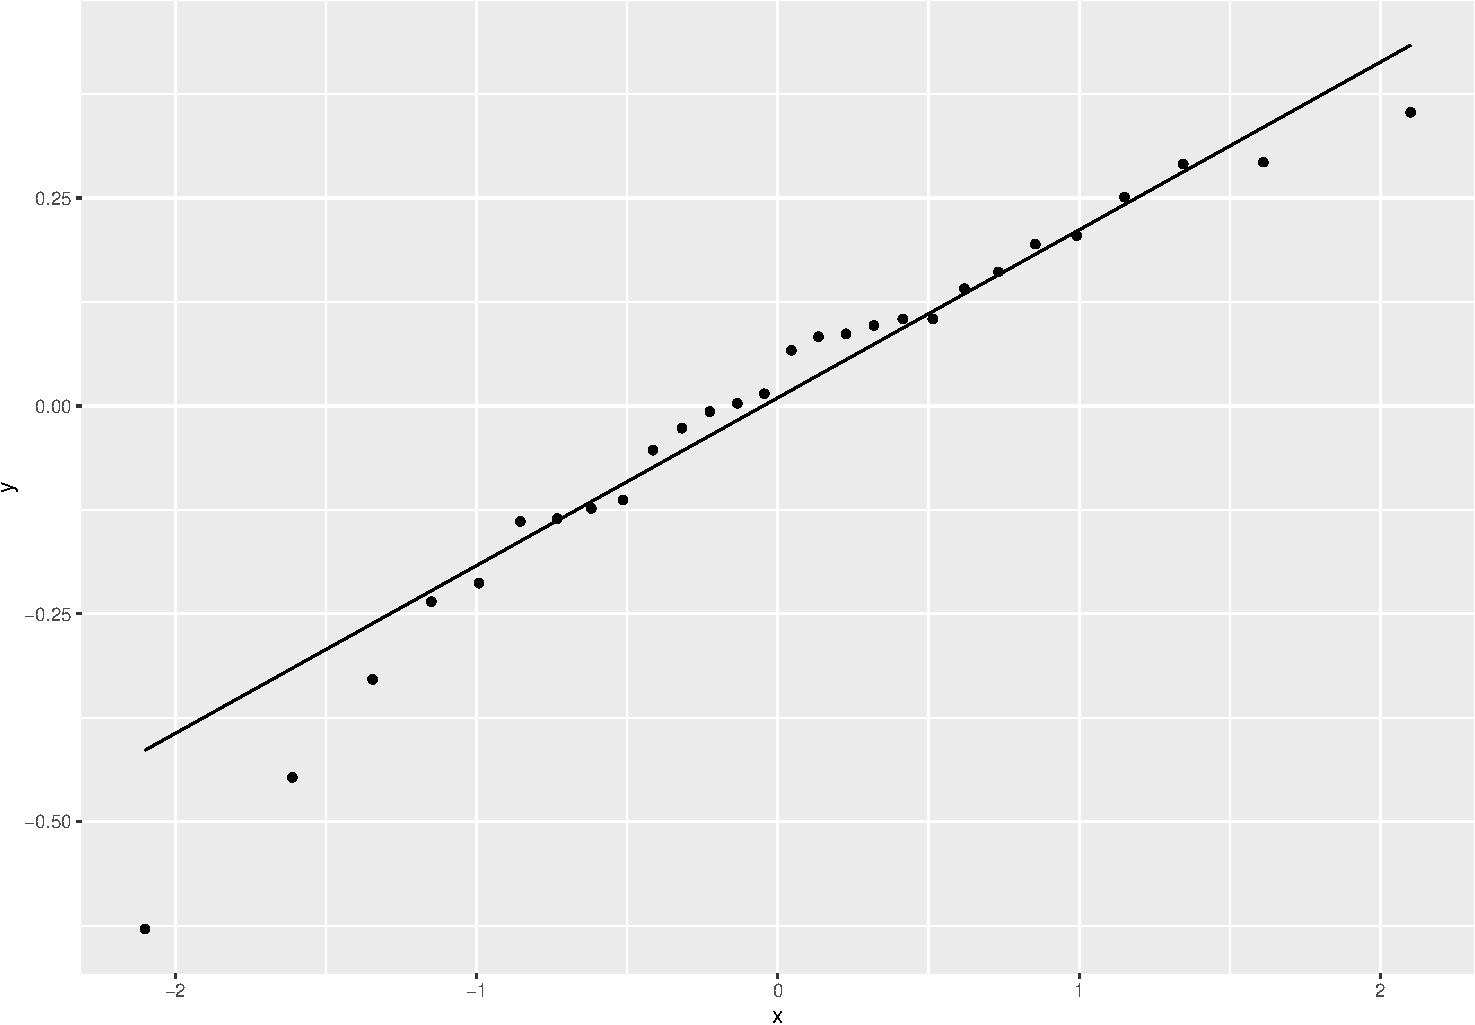
\includegraphics{anova_files/figure-beamer/bAnova-18-1.pdf}
\end{frame}

\begin{frame}[fragile]{Residuals against fitted}
\protect\hypertarget{residuals-against-fitted}{}
\begin{Shaded}
\begin{Highlighting}[]
\FunctionTok{ggplot}\NormalTok{(vitaminb}\FloatTok{.3}\NormalTok{, }\FunctionTok{aes}\NormalTok{(}\AttributeTok{x=}\NormalTok{.fitted, }\AttributeTok{y=}\NormalTok{.resid)) }\SpecialCharTok{+} \FunctionTok{geom\_point}\NormalTok{()}
\end{Highlighting}
\end{Shaded}

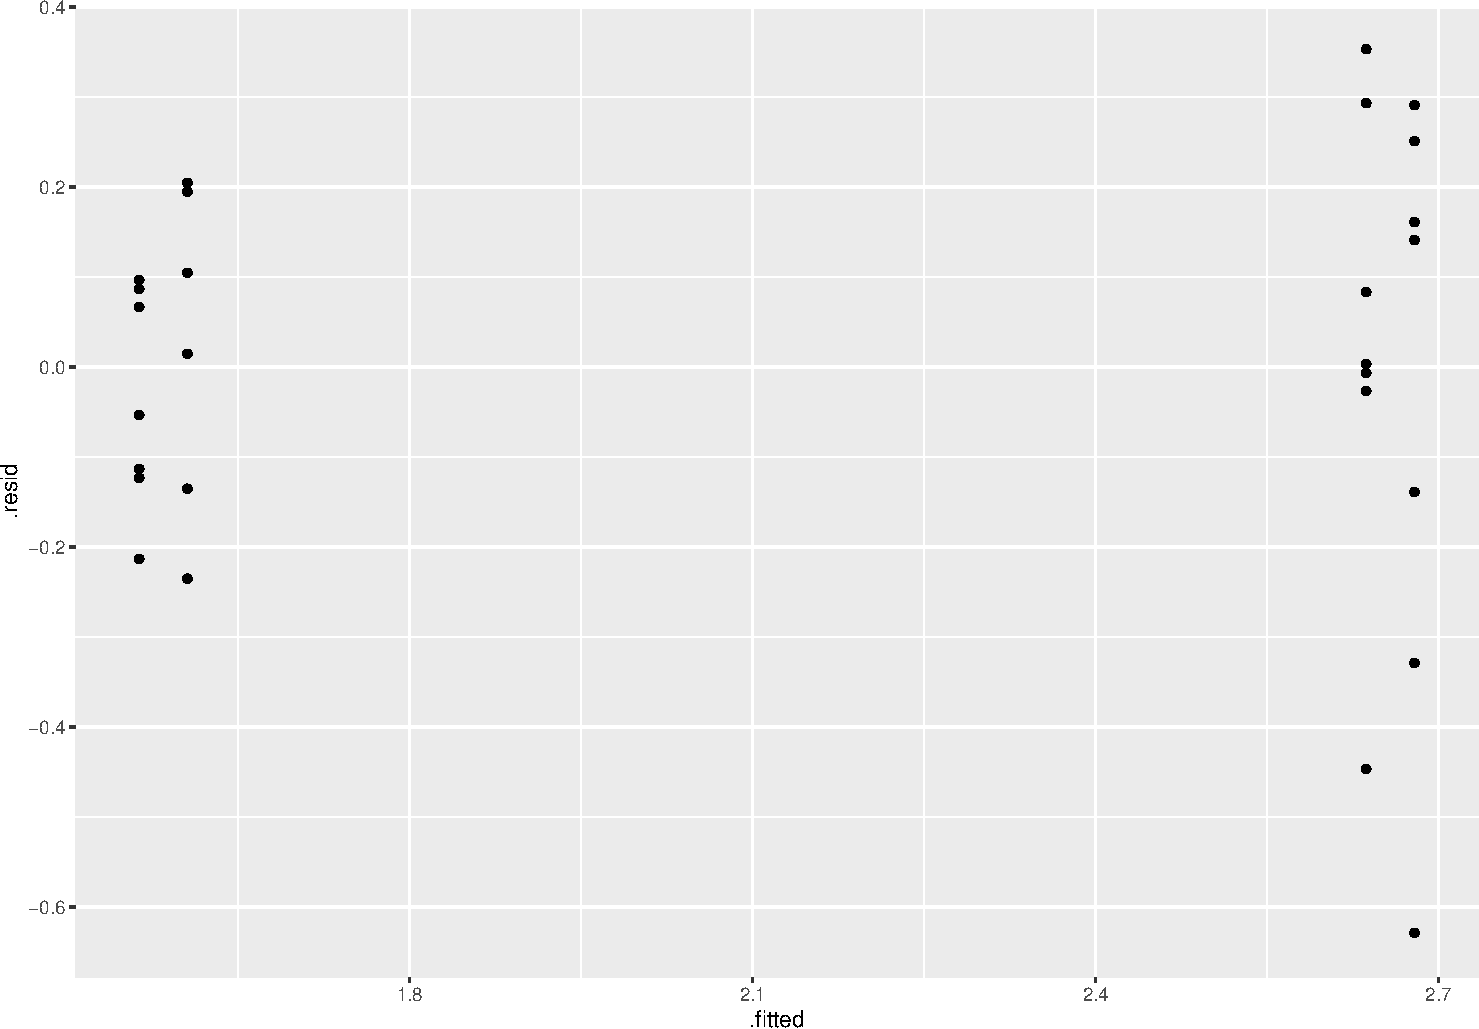
\includegraphics{anova_files/figure-beamer/bAnova-19-1.pdf}
\end{frame}

\begin{frame}[fragile]{Comments}
\protect\hypertarget{comments-1}{}
\begin{itemize}
\tightlist
\item
  2 rat sizes, 2 diets: only \(2 \times 2 = 4\) different fitted values
\item
  larger fitted values have greater spread (fan-out, transformation?)
\item
  add residuals to data to plot residuals against size, diet
  (\texttt{augment} from \texttt{broom}):
\end{itemize}

\begin{Shaded}
\begin{Highlighting}[]
\NormalTok{vitaminb}\FloatTok{.3} \SpecialCharTok{\%\textgreater{}\%} \FunctionTok{augment}\NormalTok{(vitaminb) }\OtherTok{{-}\textgreater{}}\NormalTok{ vitaminb}\FloatTok{.3}\NormalTok{a}
\end{Highlighting}
\end{Shaded}

\begin{itemize}
\tightlist
\item
  explanatory \texttt{ratsize}, \texttt{diet} categorical, so plot resid
  vs.~them with \emph{boxplots}.
\end{itemize}
\end{frame}

\begin{frame}[fragile]{Residuals vs rat size}
\protect\hypertarget{residuals-vs-rat-size}{}
\begin{Shaded}
\begin{Highlighting}[]
\FunctionTok{ggplot}\NormalTok{(vitaminb}\FloatTok{.3}\NormalTok{a, }\FunctionTok{aes}\NormalTok{(}\AttributeTok{x =}\NormalTok{ ratsize, }\AttributeTok{y =}\NormalTok{ .resid)) }\SpecialCharTok{+} 
  \FunctionTok{geom\_boxplot}\NormalTok{()}
\end{Highlighting}
\end{Shaded}

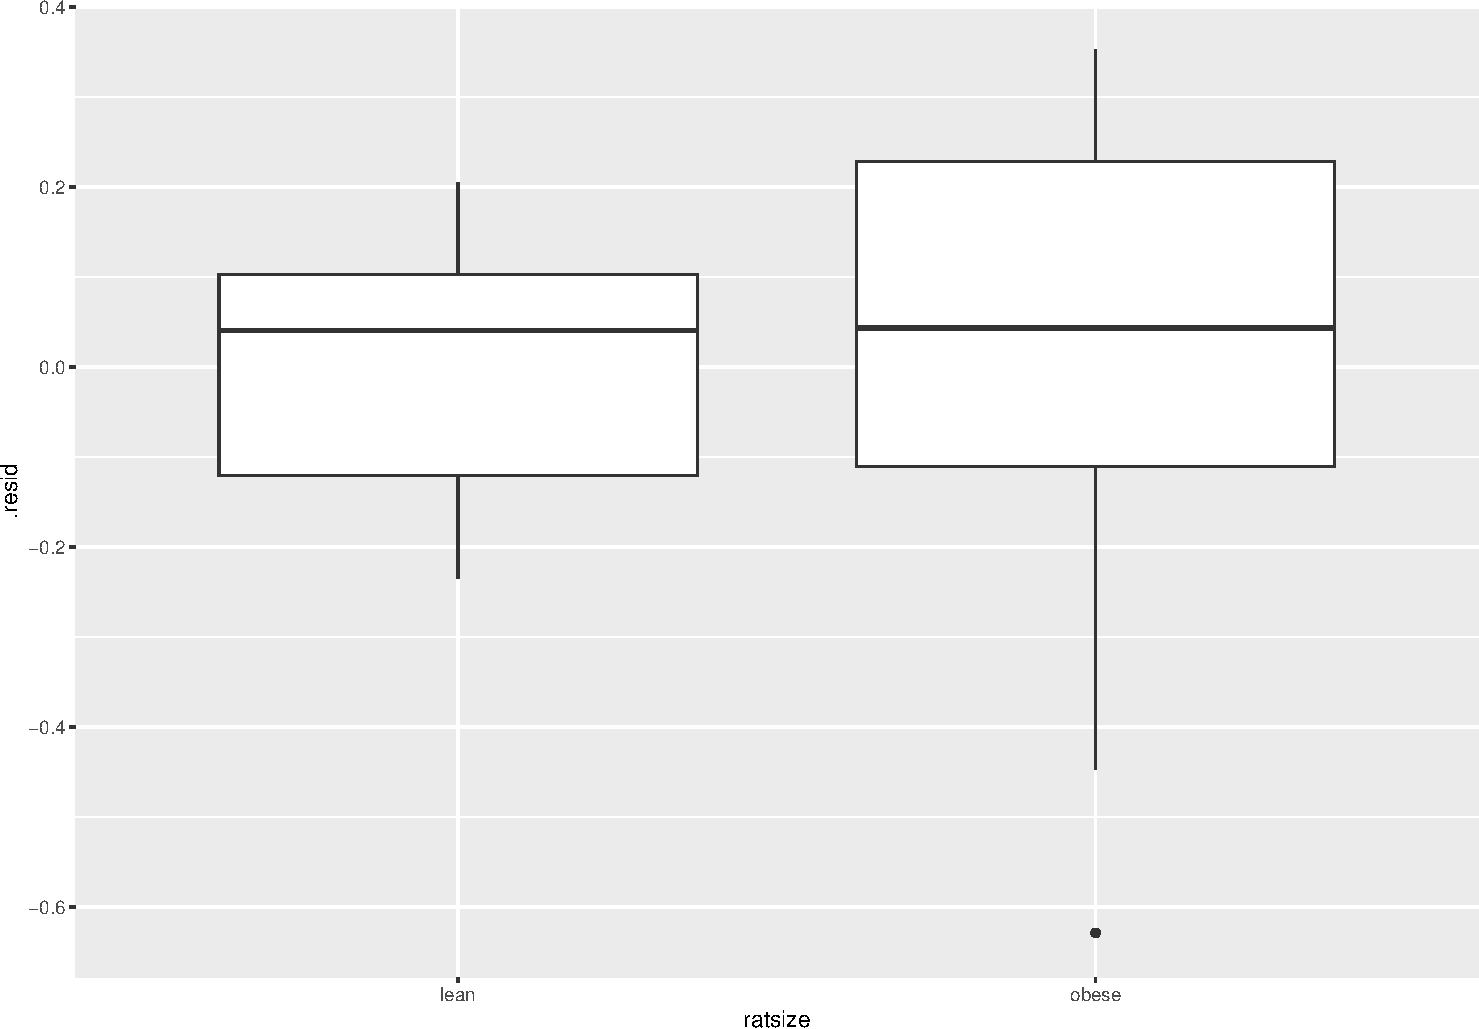
\includegraphics{anova_files/figure-beamer/bAnova-21-1.pdf}
\end{frame}

\begin{frame}[fragile]{Residuals vs diet}
\protect\hypertarget{residuals-vs-diet}{}
\begin{Shaded}
\begin{Highlighting}[]
\FunctionTok{ggplot}\NormalTok{(vitaminb}\FloatTok{.3}\NormalTok{a, }\FunctionTok{aes}\NormalTok{(}\AttributeTok{x =}\NormalTok{ diet, }\AttributeTok{y =}\NormalTok{ .resid)) }\SpecialCharTok{+} 
  \FunctionTok{geom\_boxplot}\NormalTok{()}
\end{Highlighting}
\end{Shaded}

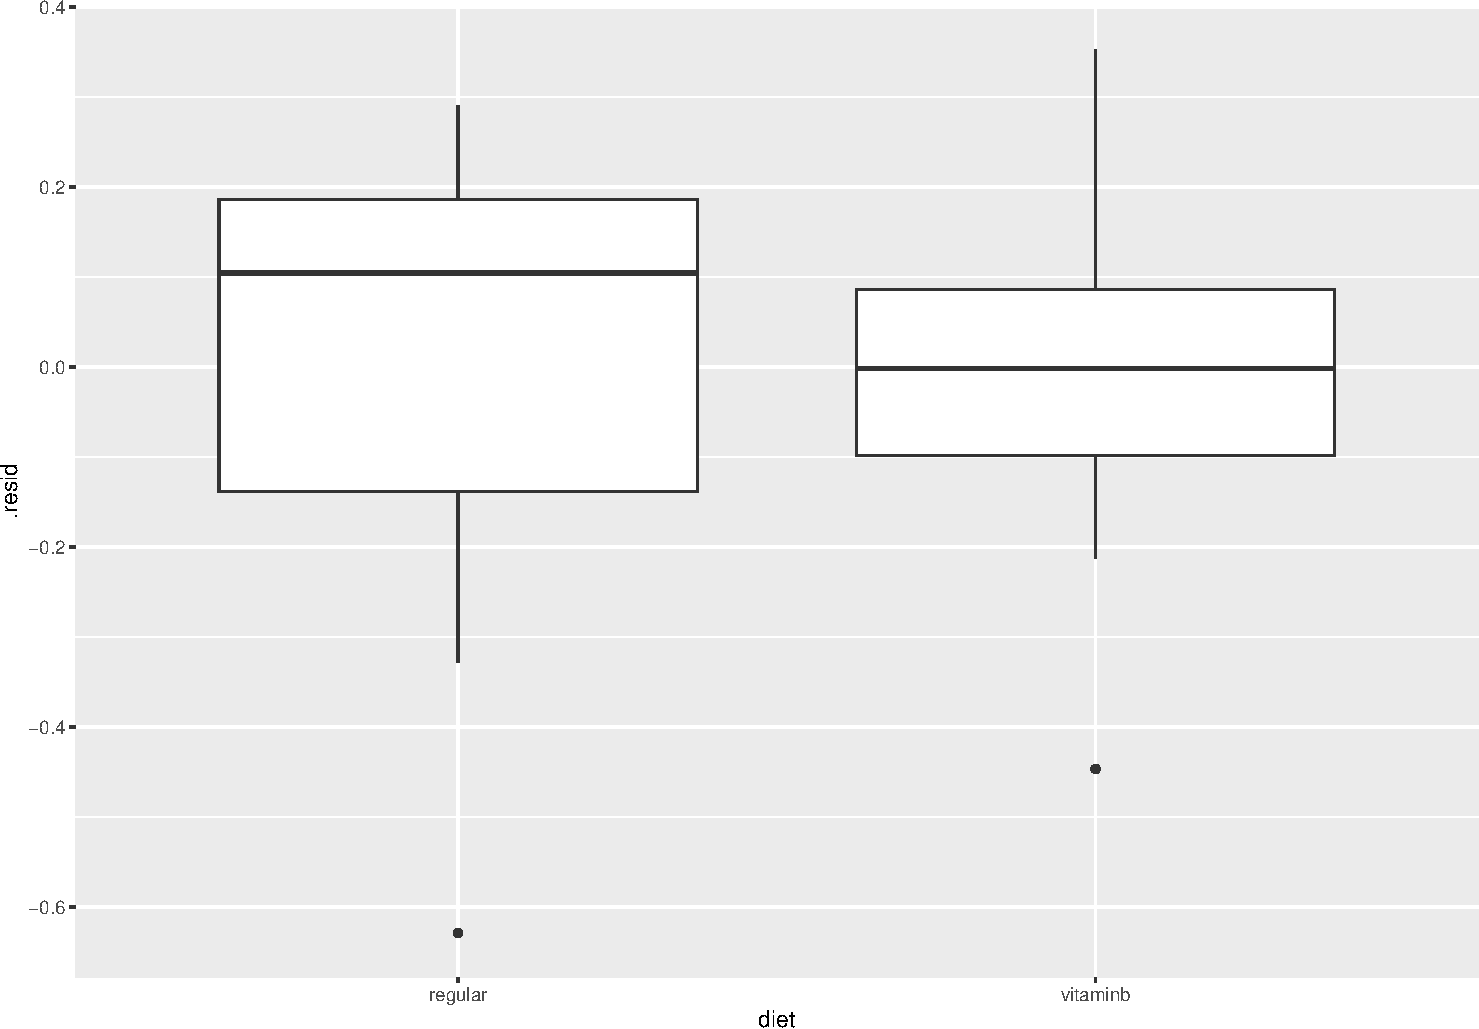
\includegraphics{anova_files/figure-beamer/bAnova-22-1.pdf}
\end{frame}

\begin{frame}{Comments}
\protect\hypertarget{comments-2}{}
\begin{itemize}
\tightlist
\item
  there are low outliers on the plot against diet
\item
  residuals for obese rats seem more spread out than for lean rats
\item
  case for transformation of rat weights
\item
  however, story from our analysis very clear:

  \begin{itemize}
  \tightlist
  \item
    rat size strongly significant
  \item
    diet nowhere near significant
  \end{itemize}
\item
  and so expect transformation to make no difference to conclusions.
\end{itemize}
\end{frame}

\begin{frame}[fragile]{The auto noise data}
\protect\hypertarget{the-auto-noise-data}{}
In 1973, the President of Texaco cited an automobile filter developed by
Associated Octel Company as effective in reducing pollution. However,
questions had been raised about the effects of filter silencing. He
referred to the data included in the report (and below) as evidence that
the silencing properties of the Octel filter were at least equal to
those of standard silencers.

\begin{Shaded}
\begin{Highlighting}[]
\NormalTok{u }\OtherTok{\textless{}{-}} \StringTok{"http://ritsokiguess.site/datafiles/autonoise.txt"}
\NormalTok{autonoise }\OtherTok{\textless{}{-}} \FunctionTok{read\_table}\NormalTok{(u)}
\end{Highlighting}
\end{Shaded}
\end{frame}

\begin{frame}[fragile]{The data}
\protect\hypertarget{the-data-2}{}
\begin{Shaded}
\begin{Highlighting}[]
\NormalTok{autonoise}
\end{Highlighting}
\end{Shaded}

\begin{verbatim}
# A tibble: 36 x 4
   noise size  type  side 
   <dbl> <chr> <chr> <chr>
 1   840 M     Std   R    
 2   770 L     Octel L    
 3   820 M     Octel R    
 4   775 L     Octel R    
 5   825 M     Octel L    
 6   840 M     Std   R    
 7   845 M     Std   L    
 8   825 M     Octel L    
 9   815 M     Octel L    
10   845 M     Std   R    
# i 26 more rows
\end{verbatim}
\end{frame}

\begin{frame}[fragile]{Making boxplot}
\protect\hypertarget{making-boxplot}{}
\begin{itemize}
\item
  Make a boxplot, but have combinations of filter type and engine size.
\item
  Use grouped boxplot again, thus:
\end{itemize}

\begin{Shaded}
\begin{Highlighting}[]
\NormalTok{g }\OtherTok{\textless{}{-}}\NormalTok{ autonoise }\SpecialCharTok{\%\textgreater{}\%}
  \FunctionTok{ggplot}\NormalTok{(}\FunctionTok{aes}\NormalTok{(}\AttributeTok{x =}\NormalTok{ size, }\AttributeTok{y =}\NormalTok{ noise, }\AttributeTok{fill =}\NormalTok{ type)) }\SpecialCharTok{+}
  \FunctionTok{geom\_boxplot}\NormalTok{()}
\end{Highlighting}
\end{Shaded}
\end{frame}

\begin{frame}[fragile]{The boxplot}
\protect\hypertarget{the-boxplot}{}
\begin{itemize}
\item
  See difference in engine noise between Octel and standard is larger
  for medium engine size than for large or small.
\item
  Some evidence of differences in spreads (ignore for now):
\end{itemize}

\begin{Shaded}
\begin{Highlighting}[]
\NormalTok{g}
\end{Highlighting}
\end{Shaded}

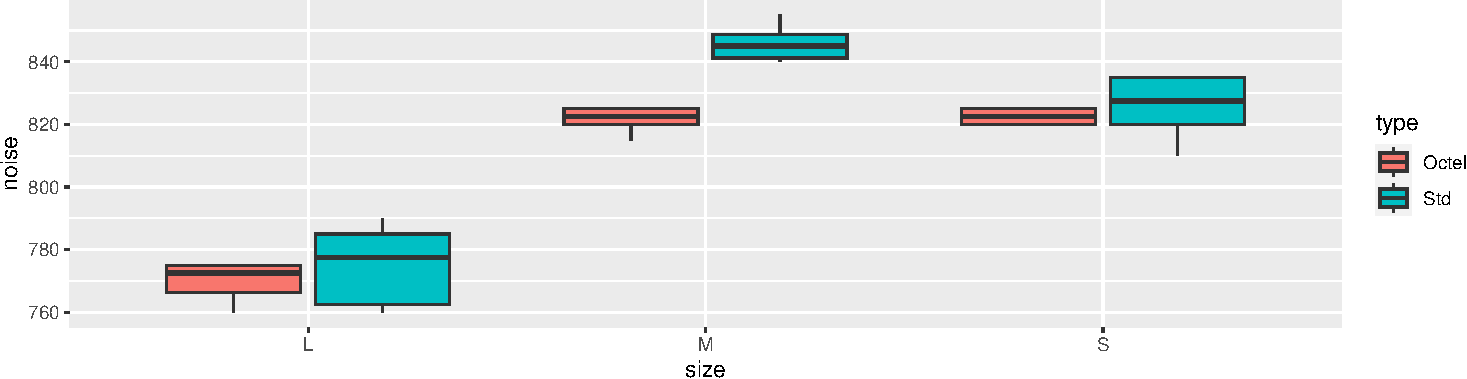
\includegraphics{anova_files/figure-beamer/bAnova-26-1.pdf}
\end{frame}

\begin{frame}[fragile]{ANOVA}
\protect\hypertarget{anova}{}
\small

\begin{Shaded}
\begin{Highlighting}[]
\NormalTok{autonoise}\FloatTok{.1} \OtherTok{\textless{}{-}} \FunctionTok{aov}\NormalTok{(noise }\SpecialCharTok{\textasciitilde{}}\NormalTok{ size }\SpecialCharTok{*}\NormalTok{ type, }\AttributeTok{data =}\NormalTok{ autonoise)}
\FunctionTok{summary}\NormalTok{(autonoise}\FloatTok{.1}\NormalTok{)}
\end{Highlighting}
\end{Shaded}

\begin{verbatim}
            Df Sum Sq Mean Sq F value   Pr(>F)    
size         2  26051   13026 199.119  < 2e-16 ***
type         1   1056    1056  16.146 0.000363 ***
size:type    2    804     402   6.146 0.005792 ** 
Residuals   30   1963      65                     
---
Signif. codes:  0 '***' 0.001 '**' 0.01 '*' 0.05 '.' 0.1 ' ' 1
\end{verbatim}

\normalsize

\begin{itemize}
\item
  The interaction is significant, as we suspected from the boxplots.
\item
  The within-group spreads don't look very equal, but only based on 6
  obs each.
\end{itemize}
\end{frame}

\begin{frame}[fragile]{Tukey: ouch!}
\protect\hypertarget{tukey-ouch}{}
\scriptsize

\begin{Shaded}
\begin{Highlighting}[]
\NormalTok{autonoise}\FloatTok{.2} \OtherTok{\textless{}{-}} \FunctionTok{TukeyHSD}\NormalTok{(autonoise}\FloatTok{.1}\NormalTok{)}
\NormalTok{autonoise}\FloatTok{.2}\SpecialCharTok{$}\StringTok{\textasciigrave{}}\AttributeTok{size:type}\StringTok{\textasciigrave{}}
\end{Highlighting}
\end{Shaded}

\begin{verbatim}
                       diff        lwr        upr        p adj
M:Octel-L:Octel  51.6666667  37.463511  65.869823 6.033496e-11
S:Octel-L:Octel  52.5000000  38.296844  66.703156 4.089762e-11
L:Std-L:Octel     5.0000000  -9.203156  19.203156 8.890358e-01
M:Std-L:Octel    75.8333333  61.630177  90.036489 4.962697e-14
S:Std-L:Octel    55.8333333  41.630177  70.036489 9.002910e-12
S:Octel-M:Octel   0.8333333 -13.369823  15.036489 9.999720e-01
L:Std-M:Octel   -46.6666667 -60.869823 -32.463511 6.766649e-10
M:Std-M:Octel    24.1666667   9.963511  38.369823 1.908995e-04
S:Std-M:Octel     4.1666667 -10.036489  18.369823 9.454142e-01
L:Std-S:Octel   -47.5000000 -61.703156 -33.296844 4.477636e-10
M:Std-S:Octel    23.3333333   9.130177  37.536489 3.129974e-04
S:Std-S:Octel     3.3333333 -10.869823  17.536489 9.787622e-01
M:Std-L:Std      70.8333333  56.630177  85.036489 6.583623e-14
S:Std-L:Std      50.8333333  36.630177  65.036489 8.937329e-11
S:Std-M:Std     -20.0000000 -34.203156  -5.796844 2.203265e-03
\end{verbatim}

\normalsize
\end{frame}

\begin{frame}[fragile]{Interaction plot}
\protect\hypertarget{interaction-plot-1}{}
\begin{itemize}
\item
  This time, don't have summary of mean noise for each size-type
  combination.
\item
  One way is to compute summaries (means) first, and feed into
  \texttt{ggplot} as in vitamin B example.
\item
  Or, have \texttt{ggplot} compute them for us, thus:
\end{itemize}

\begin{Shaded}
\begin{Highlighting}[]
\NormalTok{g }\OtherTok{\textless{}{-}} \FunctionTok{ggplot}\NormalTok{(autonoise, }\FunctionTok{aes}\NormalTok{(}
  \AttributeTok{x =}\NormalTok{ size, }\AttributeTok{y =}\NormalTok{ noise,}
  \AttributeTok{colour =}\NormalTok{ type, }\AttributeTok{group =}\NormalTok{ type}
\NormalTok{)) }\SpecialCharTok{+}
  \FunctionTok{stat\_summary}\NormalTok{(}\AttributeTok{fun =}\NormalTok{ mean, }\AttributeTok{geom =} \StringTok{"point"}\NormalTok{) }\SpecialCharTok{+}
  \FunctionTok{stat\_summary}\NormalTok{(}\AttributeTok{fun =}\NormalTok{ mean, }\AttributeTok{geom =} \StringTok{"line"}\NormalTok{)}
\end{Highlighting}
\end{Shaded}
\end{frame}

\begin{frame}[fragile]{Interaction plot}
\protect\hypertarget{interaction-plot-2}{}
The lines are definitely \emph{not} parallel, showing that the effect of
\texttt{type} is different for medium-sized engines than for others:

\begin{Shaded}
\begin{Highlighting}[]
\NormalTok{g}
\end{Highlighting}
\end{Shaded}

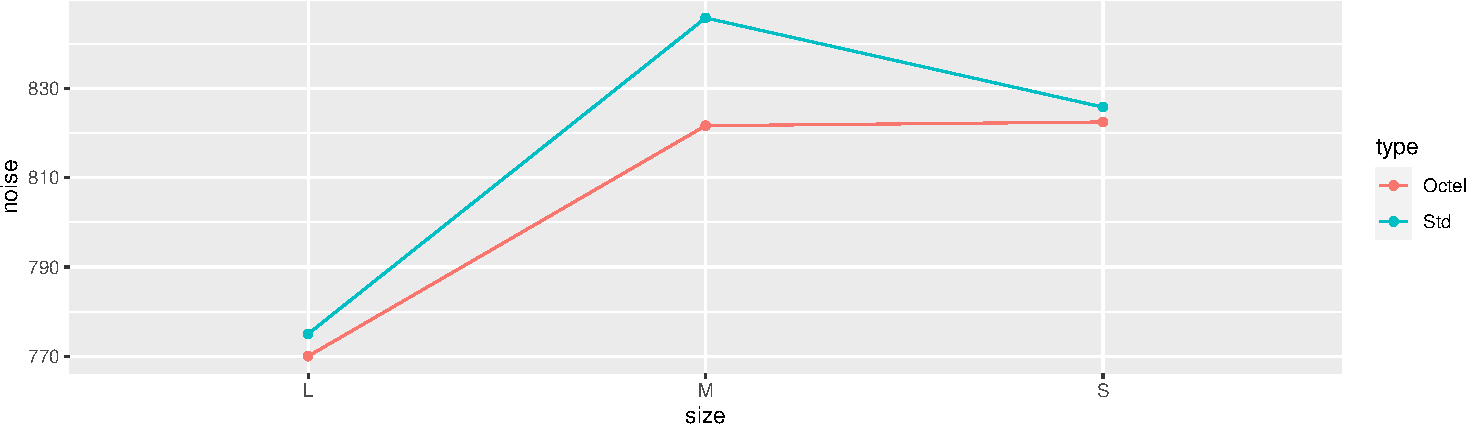
\includegraphics{anova_files/figure-beamer/bAnova-30-1.pdf}
\end{frame}

\begin{frame}[fragile]{If you don't like that\ldots}
\protect\hypertarget{if-you-dont-like-that}{}
\ldots then compute the means first, in a pipeline:

\footnotesize

\begin{Shaded}
\begin{Highlighting}[]
\NormalTok{autonoise }\SpecialCharTok{\%\textgreater{}\%}
  \FunctionTok{group\_by}\NormalTok{(size, type) }\SpecialCharTok{\%\textgreater{}\%}
  \FunctionTok{summarize}\NormalTok{(}\AttributeTok{mean\_noise =} \FunctionTok{mean}\NormalTok{(noise)) }\SpecialCharTok{\%\textgreater{}\%}
  \FunctionTok{ggplot}\NormalTok{(}\FunctionTok{aes}\NormalTok{(}
    \AttributeTok{x =}\NormalTok{ size, }\AttributeTok{y =}\NormalTok{ mean\_noise, }\AttributeTok{group =}\NormalTok{ type,}
    \AttributeTok{colour =}\NormalTok{ type}
\NormalTok{  )) }\SpecialCharTok{+} \FunctionTok{geom\_point}\NormalTok{() }\SpecialCharTok{+} \FunctionTok{geom\_line}\NormalTok{()}
\end{Highlighting}
\end{Shaded}

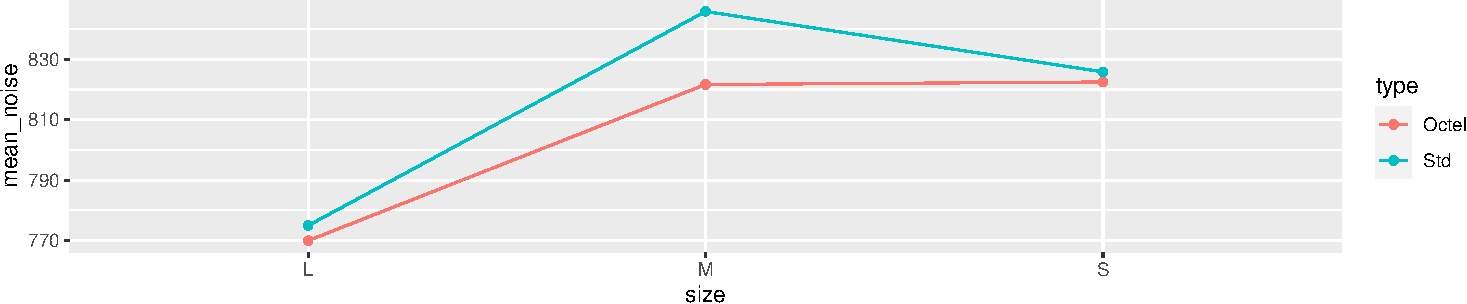
\includegraphics{anova_files/figure-beamer/bAnova-31-1.pdf}

\normalsize
\end{frame}

\begin{frame}{Simple effects for auto noise example}
\protect\hypertarget{simple-effects-for-auto-noise-example}{}
\begin{itemize}
\item
  In auto noise example, weren't interested in all comparisons between
  car size and filter type combinations.
\item
  Wanted to demonstrate (lack of) difference between filter types
  \emph{for each car type}.
\item
  These are called \textbf{simple effects} of one variable (filter type)
  conditional on other variable (car type).
\item
  To do this, pull out just the data for small cars, compare noise for
  the two filter types. Then repeat for medium and large cars. (Three
  one-way ANOVAs.)
\end{itemize}
\end{frame}

\begin{frame}[fragile]{Do it using \texttt{dplyr\ tools}}
\protect\hypertarget{do-it-using-dplyr-tools}{}
\begin{itemize}
\tightlist
\item
  Small cars:
\end{itemize}

\begin{Shaded}
\begin{Highlighting}[]
\NormalTok{autonoise }\SpecialCharTok{\%\textgreater{}\%}
  \FunctionTok{filter}\NormalTok{(size }\SpecialCharTok{==} \StringTok{"S"}\NormalTok{) }\SpecialCharTok{\%\textgreater{}\%}
  \FunctionTok{aov}\NormalTok{(noise }\SpecialCharTok{\textasciitilde{}}\NormalTok{ type, }\AttributeTok{data =}\NormalTok{ .) }\SpecialCharTok{\%\textgreater{}\%}
  \FunctionTok{summary}\NormalTok{()}
\end{Highlighting}
\end{Shaded}

\begin{verbatim}
            Df Sum Sq Mean Sq F value Pr(>F)
type         1   33.3   33.33   0.548  0.476
Residuals   10  608.3   60.83               
\end{verbatim}

\begin{itemize}
\item
  No filter difference for small cars.
\item
  For Medium, change \texttt{S} to \texttt{M} and repeat.
\end{itemize}
\end{frame}

\begin{frame}[fragile]{Simple effect of filter type for medium cars}
\protect\hypertarget{simple-effect-of-filter-type-for-medium-cars}{}
\small

\begin{Shaded}
\begin{Highlighting}[]
\NormalTok{autonoise }\SpecialCharTok{\%\textgreater{}\%}
  \FunctionTok{filter}\NormalTok{(size }\SpecialCharTok{==} \StringTok{"M"}\NormalTok{) }\SpecialCharTok{\%\textgreater{}\%}
  \FunctionTok{aov}\NormalTok{(noise }\SpecialCharTok{\textasciitilde{}}\NormalTok{ type, }\AttributeTok{data =}\NormalTok{ .) }\SpecialCharTok{\%\textgreater{}\%}
  \FunctionTok{summary}\NormalTok{()}
\end{Highlighting}
\end{Shaded}

\begin{verbatim}
            Df Sum Sq Mean Sq F value   Pr(>F)    
type         1 1752.1  1752.1   68.93 8.49e-06 ***
Residuals   10  254.2    25.4                     
---
Signif. codes:  0 '***' 0.001 '**' 0.01 '*' 0.05 '.' 0.1 ' ' 1
\end{verbatim}

\normalsize

\begin{itemize}
\tightlist
\item
  There \emph{is} an effect of filter type for medium cars. Look at
  means to investigate (over).
\end{itemize}
\end{frame}

\begin{frame}[fragile]{Mean noise for each filter type}
\protect\hypertarget{mean-noise-for-each-filter-type}{}
\ldots for medium engine size:

\begin{Shaded}
\begin{Highlighting}[]
\NormalTok{autonoise }\SpecialCharTok{\%\textgreater{}\%}
  \FunctionTok{filter}\NormalTok{(size }\SpecialCharTok{==} \StringTok{"M"}\NormalTok{) }\SpecialCharTok{\%\textgreater{}\%}
  \FunctionTok{group\_by}\NormalTok{(type) }\SpecialCharTok{\%\textgreater{}\%}
  \FunctionTok{summarize}\NormalTok{(}\AttributeTok{m =} \FunctionTok{mean}\NormalTok{(noise))}
\end{Highlighting}
\end{Shaded}

\begin{verbatim}
# A tibble: 2 x 2
  type      m
  <chr> <dbl>
1 Octel  822.
2 Std    846.
\end{verbatim}

\begin{itemize}
\tightlist
\item
  Octel filters produce \emph{less} noise for medium cars.
\end{itemize}
\end{frame}

\begin{frame}[fragile]{Large cars}
\protect\hypertarget{large-cars}{}
\begin{itemize}
\tightlist
\item
  Large cars:
\end{itemize}

\begin{Shaded}
\begin{Highlighting}[]
\NormalTok{autonoise }\SpecialCharTok{\%\textgreater{}\%}
  \FunctionTok{filter}\NormalTok{(size }\SpecialCharTok{==} \StringTok{"L"}\NormalTok{) }\SpecialCharTok{\%\textgreater{}\%}
  \FunctionTok{aov}\NormalTok{(noise }\SpecialCharTok{\textasciitilde{}}\NormalTok{ type, }\AttributeTok{data =}\NormalTok{ .) }\SpecialCharTok{\%\textgreater{}\%}
  \FunctionTok{summary}\NormalTok{()}
\end{Highlighting}
\end{Shaded}

\begin{verbatim}
            Df Sum Sq Mean Sq F value Pr(>F)
type         1     75      75   0.682  0.428
Residuals   10   1100     110               
\end{verbatim}

\begin{itemize}
\tightlist
\item
  No significant difference again.
\end{itemize}
\end{frame}

\begin{frame}[fragile]{All at once, using split/apply/combine}
\protect\hypertarget{all-at-once-using-splitapplycombine}{}
The ``split'' part:

\begin{Shaded}
\begin{Highlighting}[]
\NormalTok{autonoise }\SpecialCharTok{\%\textgreater{}\%}
  \FunctionTok{group\_by}\NormalTok{(size) }\SpecialCharTok{\%\textgreater{}\%}
  \FunctionTok{nest}\NormalTok{()}
\end{Highlighting}
\end{Shaded}

\begin{verbatim}
# A tibble: 3 x 2
# Groups:   size [3]
  size  data             
  <chr> <list>           
1 M     <tibble [12 x 3]>
2 L     <tibble [12 x 3]>
3 S     <tibble [12 x 3]>
\end{verbatim}

Now have \emph{three} rows, with the data frame for each size encoded as
\emph{one element} of this data frame.
\end{frame}

\begin{frame}[fragile]{Apply}
\protect\hypertarget{apply}{}
\begin{itemize}
\tightlist
\item
  Write function to do \texttt{aov} on a data frame with columns
  \texttt{noise} and \texttt{type}, returning P-value:
\end{itemize}

\begin{Shaded}
\begin{Highlighting}[]
\NormalTok{aov\_pval }\OtherTok{\textless{}{-}} \ControlFlowTok{function}\NormalTok{(x) \{}
\NormalTok{  noise}\FloatTok{.1} \OtherTok{\textless{}{-}} \FunctionTok{aov}\NormalTok{(noise }\SpecialCharTok{\textasciitilde{}}\NormalTok{ type, }\AttributeTok{data =}\NormalTok{ x)}
\NormalTok{  gg }\OtherTok{\textless{}{-}} \FunctionTok{tidy}\NormalTok{(noise}\FloatTok{.1}\NormalTok{)}
\NormalTok{  gg}\SpecialCharTok{$}\NormalTok{p.value[}\DecValTok{1}\NormalTok{]}
\NormalTok{\}}
\end{Highlighting}
\end{Shaded}

\begin{itemize}
\tightlist
\item
  Test it:
\end{itemize}

\begin{Shaded}
\begin{Highlighting}[]
\NormalTok{autonoise }\SpecialCharTok{\%\textgreater{}\%}
  \FunctionTok{filter}\NormalTok{(size }\SpecialCharTok{==} \StringTok{"L"}\NormalTok{) }\SpecialCharTok{\%\textgreater{}\%}
  \FunctionTok{aov\_pval}\NormalTok{()}
\end{Highlighting}
\end{Shaded}

\begin{verbatim}
[1] 0.428221
\end{verbatim}

\begin{itemize}
\tightlist
\item
  Check.
\end{itemize}
\end{frame}

\begin{frame}[fragile]{Combine}
\protect\hypertarget{combine}{}
\begin{itemize}
\tightlist
\item
  Apply this function to each of the nested data frames (one per engine
  size):
\end{itemize}

\begin{Shaded}
\begin{Highlighting}[]
\NormalTok{autonoise }\SpecialCharTok{\%\textgreater{}\%}
  \FunctionTok{nest\_by}\NormalTok{(size) }\SpecialCharTok{\%\textgreater{}\%} 
  \FunctionTok{rowwise}\NormalTok{() }\SpecialCharTok{\%\textgreater{}\%} 
  \FunctionTok{mutate}\NormalTok{(}\AttributeTok{p\_val =} \FunctionTok{aov\_pval}\NormalTok{(data))}
\end{Highlighting}
\end{Shaded}

\begin{verbatim}
# A tibble: 3 x 3
# Rowwise: 
  size                data      p_val
  <chr> <list<tibble[,3]>>      <dbl>
1 L               [12 x 3] 0.428     
2 M               [12 x 3] 0.00000849
3 S               [12 x 3] 0.476     
\end{verbatim}
\end{frame}

\begin{frame}[fragile]{Tidy up}
\protect\hypertarget{tidy-up}{}
\begin{itemize}
\tightlist
\item
  The \texttt{data} column was stepping-stone to getting answer. Don't
  need it any more:
\end{itemize}

\small

\begin{Shaded}
\begin{Highlighting}[]
\NormalTok{autonoise }\SpecialCharTok{\%\textgreater{}\%}
  \FunctionTok{nest\_by}\NormalTok{(size) }\SpecialCharTok{\%\textgreater{}\%} 
  \FunctionTok{rowwise}\NormalTok{() }\SpecialCharTok{\%\textgreater{}\%} 
  \FunctionTok{mutate}\NormalTok{(}\AttributeTok{p\_val =} \FunctionTok{aov\_pval}\NormalTok{(data)) }\SpecialCharTok{\%\textgreater{}\%} 
  \FunctionTok{select}\NormalTok{(}\SpecialCharTok{{-}}\NormalTok{data) }\OtherTok{{-}\textgreater{}}\NormalTok{ simple\_effects}
\NormalTok{simple\_effects}
\end{Highlighting}
\end{Shaded}

\begin{verbatim}
# A tibble: 3 x 2
# Rowwise: 
  size       p_val
  <chr>      <dbl>
1 L     0.428     
2 M     0.00000849
3 S     0.476     
\end{verbatim}

\normalsize
\end{frame}

\begin{frame}[fragile]{Simultaneous tests}
\protect\hypertarget{simultaneous-tests}{}
\begin{itemize}
\tightlist
\item
  When testing simple effects, doing several tests at once. (In this
  case, 3.) Have to adjust P-values for this. Eg.~Holm:
\end{itemize}

\footnotesize

\begin{Shaded}
\begin{Highlighting}[]
\NormalTok{simple\_effects }\SpecialCharTok{\%\textgreater{}\%} \FunctionTok{ungroup}\NormalTok{() }\SpecialCharTok{\%\textgreater{}\%} \FunctionTok{arrange}\NormalTok{(p\_val) }\SpecialCharTok{\%\textgreater{}\%}
  \FunctionTok{mutate}\NormalTok{(}\AttributeTok{multiplier =} \DecValTok{4} \SpecialCharTok{{-}} \FunctionTok{row\_number}\NormalTok{()) }\SpecialCharTok{\%\textgreater{}\%}
  \FunctionTok{mutate}\NormalTok{(}\AttributeTok{p\_val\_adj =}\NormalTok{ p\_val }\SpecialCharTok{*}\NormalTok{ multiplier)}
\end{Highlighting}
\end{Shaded}

\begin{verbatim}
# A tibble: 3 x 4
  size       p_val multiplier p_val_adj
  <chr>      <dbl>      <dbl>     <dbl>
1 M     0.00000849          3 0.0000255
2 L     0.428               2 0.856    
3 S     0.476               1 0.476    
\end{verbatim}

\normalsize

\footnotesize

\begin{itemize}
\item
  No change in rejection decisions.
\item
  Octel filters sig.~better in terms of noise for medium cars, and not
  sig.~different for other sizes.
\item
  Octel filters never significantly worse than standard ones.
\end{itemize}

\normalsize
\end{frame}

\begin{frame}[fragile]{Confidence intervals}
\protect\hypertarget{confidence-intervals}{}
\begin{itemize}
\item
  Perhaps better way of assessing simple effects: look at
  \emph{confidence intervals} rather than tests.
\item
  Gives us sense of accuracy of estimation, and thus whether
  non-significance might be lack of power: ``absence of evidence is not
  evidence of absence'\,'.
\item
  Works here because \emph{two} filter types, using \texttt{t.test} for
  each engine type.
\item
  Want to show that the Octel filter is equivalent to or better than the
  standard filter, in terms of engine noise.
\end{itemize}
\end{frame}

\begin{frame}[fragile]{Equivalence and noninferiority}
\protect\hypertarget{equivalence-and-noninferiority}{}
\begin{itemize}
\item
  Known as ``equivalence testing'' in medical world. A good read:
  \href{http://www.ncbi.nlm.nih.gov/pmc/articles/PMC3019319/}{link}.
  Basic idea: decide on size of difference \(\delta\) that would be
  considered ``equivalent'', and if CI entirely inside \(\pm \delta\),
  have evidence in favour of equivalence.
\item
  We really want to show that the Octel filters are ``no worse'' than
  the standard one: that is, equivalent \emph{or better} than standard
  filters.
\item
  Such a ``noninferiority test'' done by checking that
  \texttt{upper\ limit} of CI, new minus old, is \emph{less} than
  \(\delta\). (This requires careful thinking about (i) which way around
  the difference is and (ii) whether a higher or lower value is better.)
\end{itemize}
\end{frame}

\begin{frame}[fragile]{CI for small cars}
\protect\hypertarget{ci-for-small-cars}{}
Same idea as for simple effect test:

\begin{Shaded}
\begin{Highlighting}[]
\NormalTok{autonoise }\SpecialCharTok{\%\textgreater{}\%}
  \FunctionTok{filter}\NormalTok{(size }\SpecialCharTok{==} \StringTok{"S"}\NormalTok{) }\SpecialCharTok{\%\textgreater{}\%}
  \FunctionTok{t.test}\NormalTok{(noise }\SpecialCharTok{\textasciitilde{}}\NormalTok{ type, }\AttributeTok{data =}\NormalTok{ .) }\SpecialCharTok{\%\textgreater{}\%}
  \FunctionTok{pluck}\NormalTok{(}\StringTok{"conf.int"}\NormalTok{)}
\end{Highlighting}
\end{Shaded}

\begin{verbatim}
[1] -14.517462   7.850795
attr(,"conf.level")
[1] 0.95
\end{verbatim}
\end{frame}

\begin{frame}[fragile]{CI for medium cars}
\protect\hypertarget{ci-for-medium-cars}{}
\begin{Shaded}
\begin{Highlighting}[]
\NormalTok{autonoise }\SpecialCharTok{\%\textgreater{}\%}
  \FunctionTok{filter}\NormalTok{(size }\SpecialCharTok{==} \StringTok{"M"}\NormalTok{) }\SpecialCharTok{\%\textgreater{}\%}
  \FunctionTok{t.test}\NormalTok{(noise }\SpecialCharTok{\textasciitilde{}}\NormalTok{ type, }\AttributeTok{data =}\NormalTok{ .) }\SpecialCharTok{\%\textgreater{}\%}
  \FunctionTok{pluck}\NormalTok{(}\StringTok{"conf.int"}\NormalTok{)}
\end{Highlighting}
\end{Shaded}

\begin{verbatim}
[1] -30.75784 -17.57549
attr(,"conf.level")
[1] 0.95
\end{verbatim}
\end{frame}

\begin{frame}[fragile]{CI for large cars}
\protect\hypertarget{ci-for-large-cars}{}
\begin{Shaded}
\begin{Highlighting}[]
\NormalTok{autonoise }\SpecialCharTok{\%\textgreater{}\%}
  \FunctionTok{filter}\NormalTok{(size }\SpecialCharTok{==} \StringTok{"L"}\NormalTok{) }\SpecialCharTok{\%\textgreater{}\%}
  \FunctionTok{t.test}\NormalTok{(noise }\SpecialCharTok{\textasciitilde{}}\NormalTok{ type, }\AttributeTok{data =}\NormalTok{ .) }\SpecialCharTok{\%\textgreater{}\%}
  \FunctionTok{pluck}\NormalTok{(}\StringTok{"conf.int"}\NormalTok{)}
\end{Highlighting}
\end{Shaded}

\begin{verbatim}
[1] -19.270673   9.270673
attr(,"conf.level")
[1] 0.95
\end{verbatim}
\end{frame}

\begin{frame}[fragile]{Or, all at once: split/apply/combine}
\protect\hypertarget{or-all-at-once-splitapplycombine}{}
\begin{Shaded}
\begin{Highlighting}[]
\NormalTok{ci\_func }\OtherTok{\textless{}{-}} \ControlFlowTok{function}\NormalTok{(x) \{}
\NormalTok{  tt }\OtherTok{\textless{}{-}} \FunctionTok{t.test}\NormalTok{(noise }\SpecialCharTok{\textasciitilde{}}\NormalTok{ type, }\AttributeTok{data =}\NormalTok{ x)}
\NormalTok{  tt}\SpecialCharTok{$}\NormalTok{conf.int}
\NormalTok{\}}

\NormalTok{autonoise }\SpecialCharTok{\%\textgreater{}\%} \FunctionTok{nest\_by}\NormalTok{(size) }\SpecialCharTok{\%\textgreater{}\%}
  \FunctionTok{rowwise}\NormalTok{() }\SpecialCharTok{\%\textgreater{}\%} 
  \FunctionTok{mutate}\NormalTok{(}\AttributeTok{ci =} \FunctionTok{list}\NormalTok{(}\FunctionTok{ci\_func}\NormalTok{(data))) }\SpecialCharTok{\%\textgreater{}\%}
  \FunctionTok{unnest\_wider}\NormalTok{(ci, }\AttributeTok{names\_sep =} \StringTok{"\_"}\NormalTok{) }\OtherTok{{-}\textgreater{}}\NormalTok{ cis}
\end{Highlighting}
\end{Shaded}

\normalsize
\end{frame}

\begin{frame}[fragile]{Results}
\protect\hypertarget{results}{}
\begin{Shaded}
\begin{Highlighting}[]
\NormalTok{cis }\SpecialCharTok{\%\textgreater{}\%} \FunctionTok{select}\NormalTok{(size, }\FunctionTok{starts\_with}\NormalTok{(}\StringTok{"ci"}\NormalTok{))}
\end{Highlighting}
\end{Shaded}

\begin{verbatim}
# A tibble: 3 x 3
  size   ci_1   ci_2
  <chr> <dbl>  <dbl>
1 L     -19.3   9.27
2 M     -30.8 -17.6 
3 S     -14.5   7.85
\end{verbatim}
\end{frame}

\begin{frame}[fragile]{Procedure}
\protect\hypertarget{procedure}{}
\begin{itemize}
\item
  Function to get CI of difference in noise means for types of filter on
  input data frame
\item
  Nest by \texttt{size} (mini-df \texttt{data} per size)
\item
  Calculate CI for each thing in \texttt{data}: CI is two numbers long
\item
  \texttt{unnest} \texttt{ci} column (wider) to see two numbers in each
  CI.
\end{itemize}
\end{frame}

\begin{frame}[fragile]{CIs and noninferiority test}
\protect\hypertarget{cis-and-noninferiority-test}{}
\begin{itemize}
\item
  Suppose we decide that a 20 dB difference would be considered
  equivalent. (I have no idea whether that is reasonable.)
\item
  Intervals: \vspace{2ex}
\end{itemize}

\small

\begin{Shaded}
\begin{Highlighting}[]
\NormalTok{cis }\SpecialCharTok{\%\textgreater{}\%} \FunctionTok{select}\NormalTok{(}\SpecialCharTok{{-}}\NormalTok{data)}
\end{Highlighting}
\end{Shaded}

\begin{verbatim}
# A tibble: 3 x 3
  size   ci_1   ci_2
  <chr> <dbl>  <dbl>
1 L     -19.3   9.27
2 M     -30.8 -17.6 
3 S     -14.5   7.85
\end{verbatim}

\normalsize
\end{frame}

\begin{frame}{Comments}
\protect\hypertarget{comments-3}{}
\begin{itemize}
\item
  In all cases, upper limit of CI is less than 20 dB. The Octel filters
  are ``noninferior'' to the standard ones.
\item
  Caution: we did 3 procedures at once again. The true confidence level
  is not 95\%. (Won't worry about that here.)
\end{itemize}
\end{frame}

\begin{frame}{Contrasts in ANOVA}
\protect\hypertarget{contrasts-in-anova}{}
\begin{itemize}
\item
  Sometimes, don't want to compare \emph{all} groups, only \emph{some}
  of them.
\item
  Might be able to specify these comparisons ahead of time; other
  comparisons of no interest.
\item
  Wasteful to do ANOVA and Tukey.
\end{itemize}
\end{frame}

\begin{frame}[fragile]{Example: chainsaw kickback}
\protect\hypertarget{example-chainsaw-kickback}{}
\begin{itemize}
\item
  From
  \href{http://www.ohio.edu/plantbio/staff/mccarthy/quantmet/lectures/ANOVA2.pdf}{link}.
\item
  Forest manager concerned about safety of chainsaws issued to field
  crew. 4 models of chainsaws, measure ``kickback'' (degrees of
  deflection) for 5 of each:
\end{itemize}

\begin{verbatim}

 A  B  C  D
-----------
42 28 57 29
17 50 45 29
24 44 48 22
39 32 41 34
43 61 54 30
\end{verbatim}

\begin{itemize}
\tightlist
\item
  So far, standard 1-way ANOVA: what differences are there among models?
\end{itemize}
\end{frame}

\begin{frame}{chainsaw kickback (2)}
\protect\hypertarget{chainsaw-kickback-2}{}
\begin{itemize}
\item
  But: models A and D are designed to be used at home, while models B
  and C are industrial models.
\item
  Suggests these comparisons of interest:
\item
  home vs.~industrial
\item
  the two home models A vs.~D
\item
  the two industrial models B vs.~C.
\item
  Don't need to compare \emph{all} the pairs of models.
\end{itemize}
\end{frame}

\begin{frame}{What is a contrast?}
\protect\hypertarget{what-is-a-contrast}{}
\begin{itemize}
\item
  Contrast is a linear combination of group means.
\item
  Notation: \(\mu_A\) for (population) mean of group \(A\), and so on.
\item
  In example, compare two home models: \(H_0: \mu_A-\mu_D=0\).
\item
  Compare two industrial models: \(H_0: \mu_B-\mu_C=0\).
\item
  Compare average of two home models vs.~average of two industrial
  models: \(H_0: \frac{1}{2}(\mu_A+\mu_D)-{1\over 2}(\mu_B+\mu_C)=0\) or
  \(H_0: 0.5\mu_A-0.5\mu_B-0.5\mu_C+0.5\mu_D=0\).
\item
  Note that coefficients of contrasts add to 0, and right-hand side is
  0.
\end{itemize}
\end{frame}

\begin{frame}[fragile]{Contrasts in R}
\protect\hypertarget{contrasts-in-r}{}
\begin{itemize}
\tightlist
\item
  Comparing two home models A and D (\(\mu_A-\mu_D=0\)):
\end{itemize}

\begin{Shaded}
\begin{Highlighting}[]
\NormalTok{c.home }\OtherTok{\textless{}{-}} \FunctionTok{c}\NormalTok{(}\DecValTok{1}\NormalTok{, }\DecValTok{0}\NormalTok{, }\DecValTok{0}\NormalTok{, }\SpecialCharTok{{-}}\DecValTok{1}\NormalTok{)}
\end{Highlighting}
\end{Shaded}

\begin{itemize}
\tightlist
\item
  Comparing two industrial models B and C (\(\mu_B-\mu_C=0\)):
\end{itemize}

\begin{Shaded}
\begin{Highlighting}[]
\NormalTok{c.industrial }\OtherTok{\textless{}{-}} \FunctionTok{c}\NormalTok{(}\DecValTok{0}\NormalTok{, }\DecValTok{1}\NormalTok{, }\SpecialCharTok{{-}}\DecValTok{1}\NormalTok{, }\DecValTok{0}\NormalTok{)}
\end{Highlighting}
\end{Shaded}

\begin{itemize}
\tightlist
\item
  Comparing home average vs.~industrial average
  (\(0.5\mu_A-0.5\mu_B-0.5\mu_C+0.5\mu_D=0\)):
\end{itemize}

\begin{Shaded}
\begin{Highlighting}[]
\NormalTok{c.home.ind }\OtherTok{\textless{}{-}} \FunctionTok{c}\NormalTok{(}\FloatTok{0.5}\NormalTok{, }\SpecialCharTok{{-}}\FloatTok{0.5}\NormalTok{, }\SpecialCharTok{{-}}\FloatTok{0.5}\NormalTok{, }\FloatTok{0.5}\NormalTok{)}
\end{Highlighting}
\end{Shaded}
\end{frame}

\begin{frame}[fragile]{Orthogonal contrasts}
\protect\hypertarget{orthogonal-contrasts}{}
\begin{itemize}
\tightlist
\item
  What happens if we multiply the contrast coefficients one by one?
\end{itemize}

\begin{Shaded}
\begin{Highlighting}[]
\NormalTok{c.home }\SpecialCharTok{*}\NormalTok{ c.industrial}
\end{Highlighting}
\end{Shaded}

\begin{verbatim}
[1] 0 0 0 0
\end{verbatim}

\begin{Shaded}
\begin{Highlighting}[]
\NormalTok{c.home }\SpecialCharTok{*}\NormalTok{ c.home.ind}
\end{Highlighting}
\end{Shaded}

\begin{verbatim}
[1]  0.5  0.0  0.0 -0.5
\end{verbatim}

\begin{Shaded}
\begin{Highlighting}[]
\NormalTok{c.industrial }\SpecialCharTok{*}\NormalTok{ c.home.ind}
\end{Highlighting}
\end{Shaded}

\begin{verbatim}
[1]  0.0 -0.5  0.5  0.0
\end{verbatim}

\begin{itemize}
\tightlist
\item
  in each case, the results \textbf{add up to zero}. Such contrasts are
  called \textbf{orthogonal}.
\end{itemize}
\end{frame}

\begin{frame}[fragile]{Orthogonal contrasts (2)}
\protect\hypertarget{orthogonal-contrasts-2}{}
\begin{itemize}
\tightlist
\item
  Compare these:
\end{itemize}

\normalsize

\begin{Shaded}
\begin{Highlighting}[]
\NormalTok{c1 }\OtherTok{\textless{}{-}} \FunctionTok{c}\NormalTok{(}\DecValTok{1}\NormalTok{, }\SpecialCharTok{{-}}\DecValTok{1}\NormalTok{, }\DecValTok{0}\NormalTok{)}
\NormalTok{c2 }\OtherTok{\textless{}{-}} \FunctionTok{c}\NormalTok{(}\DecValTok{0}\NormalTok{, }\DecValTok{1}\NormalTok{, }\SpecialCharTok{{-}}\DecValTok{1}\NormalTok{)}
\FunctionTok{sum}\NormalTok{(c1 }\SpecialCharTok{*}\NormalTok{ c2)}
\end{Highlighting}
\end{Shaded}

\begin{verbatim}
[1] -1
\end{verbatim}

\normalsize

Not zero, so \texttt{c1} and \texttt{c2} are \emph{not} orthogonal.

\begin{itemize}
\item
  Orthogonal contrasts are much easier to deal with.
\item
  Can use non-orthogonal contrasts, but more trouble (beyond us).
\end{itemize}
\end{frame}

\begin{frame}[fragile]{Read in data}
\protect\hypertarget{read-in-data}{}
\small

\begin{Shaded}
\begin{Highlighting}[]
\NormalTok{url }\OtherTok{\textless{}{-}} \StringTok{"http://ritsokiguess.site/datafiles/chainsaw.txt"}
\NormalTok{chain.wide }\OtherTok{\textless{}{-}} \FunctionTok{read\_table}\NormalTok{(url)}
\NormalTok{chain.wide}
\end{Highlighting}
\end{Shaded}

\begin{verbatim}
# A tibble: 5 x 4
      A     B     C     D
  <dbl> <dbl> <dbl> <dbl>
1    42    28    57    29
2    17    50    45    29
3    24    44    48    22
4    39    32    41    34
5    43    61    54    30
\end{verbatim}

\normalsize
\end{frame}

\begin{frame}[fragile]{Tidying}
\protect\hypertarget{tidying}{}
Need all the kickbacks in \emph{one} column:

\begin{Shaded}
\begin{Highlighting}[]
\NormalTok{chain.wide }\SpecialCharTok{\%\textgreater{}\%} 
  \FunctionTok{pivot\_longer}\NormalTok{(A}\SpecialCharTok{:}\NormalTok{D, }\AttributeTok{names\_to =} \StringTok{"model"}\NormalTok{, }
               \AttributeTok{names\_ptypes =} \FunctionTok{list}\NormalTok{(}\AttributeTok{model=}\FunctionTok{factor}\NormalTok{()), }
               \AttributeTok{values\_to =} \StringTok{"kickback"}\NormalTok{) }\OtherTok{{-}\textgreater{}}\NormalTok{ chain}
\end{Highlighting}
\end{Shaded}
\end{frame}

\begin{frame}[fragile]{Starting the analysis (2)}
\protect\hypertarget{starting-the-analysis-2}{}
The proper data frame:

\begin{Shaded}
\begin{Highlighting}[]
\NormalTok{chain }
\end{Highlighting}
\end{Shaded}

\begin{verbatim}
# A tibble: 20 x 2
   model kickback
   <fct>    <dbl>
 1 A           42
 2 B           28
 3 C           57
 4 D           29
 5 A           17
 6 B           50
 7 C           45
 8 D           29
 9 A           24
10 B           44
11 C           48
12 D           22
13 A           39
14 B           32
15 C           41
16 D           34
17 A           43
18 B           61
19 C           54
20 D           30
\end{verbatim}
\end{frame}

\begin{frame}[fragile]{Setting up contrasts}
\protect\hypertarget{setting-up-contrasts}{}
\begin{Shaded}
\begin{Highlighting}[]
\NormalTok{m }\OtherTok{\textless{}{-}} \FunctionTok{cbind}\NormalTok{(c.home, c.industrial, c.home.ind)}
\NormalTok{m}
\end{Highlighting}
\end{Shaded}

\begin{verbatim}
     c.home c.industrial c.home.ind
[1,]      1            0        0.5
[2,]      0            1       -0.5
[3,]      0           -1       -0.5
[4,]     -1            0        0.5
\end{verbatim}

\begin{Shaded}
\begin{Highlighting}[]
\FunctionTok{contrasts}\NormalTok{(chain}\SpecialCharTok{$}\NormalTok{model) }\OtherTok{\textless{}{-}}\NormalTok{ m}
\end{Highlighting}
\end{Shaded}
\end{frame}

\begin{frame}[fragile]{ANOVA \emph{as if regression}}
\protect\hypertarget{anova-as-if-regression}{}
\scriptsize

\begin{Shaded}
\begin{Highlighting}[]
\NormalTok{chain}\FloatTok{.1} \OtherTok{\textless{}{-}} \FunctionTok{lm}\NormalTok{(kickback }\SpecialCharTok{\textasciitilde{}}\NormalTok{ model, }\AttributeTok{data =}\NormalTok{ chain)}
\FunctionTok{summary}\NormalTok{(chain}\FloatTok{.1}\NormalTok{)}
\end{Highlighting}
\end{Shaded}

\begin{verbatim}

Call:
lm(formula = kickback ~ model, data = chain)

Residuals:
   Min     1Q Median     3Q    Max 
-16.00  -7.10   0.60   6.25  18.00 

Coefficients:
                  Estimate Std. Error t value Pr(>|t|)    
(Intercept)         38.450      2.179  17.649 6.52e-12 ***
modelc.home          2.100      3.081   0.682  0.50524    
modelc.industrial   -3.000      3.081  -0.974  0.34469    
modelc.home.ind    -15.100      4.357  -3.466  0.00319 ** 
---
Signif. codes:  0 '***' 0.001 '**' 0.01 '*' 0.05 '.' 0.1 ' ' 1

Residual standard error: 9.743 on 16 degrees of freedom
Multiple R-squared:  0.4562,    Adjusted R-squared:  0.3542 
F-statistic: 4.474 on 3 and 16 DF,  p-value: 0.01833
\end{verbatim}

\normalsize
\end{frame}

\begin{frame}[fragile]{Conclusions}
\protect\hypertarget{conclusions}{}
\begin{Shaded}
\begin{Highlighting}[]
\FunctionTok{tidy}\NormalTok{(chain}\FloatTok{.1}\NormalTok{) }\SpecialCharTok{\%\textgreater{}\%} \FunctionTok{select}\NormalTok{(term, p.value)}
\end{Highlighting}
\end{Shaded}

\begin{verbatim}
# A tibble: 4 x 2
  term               p.value
  <chr>                <dbl>
1 (Intercept)       6.52e-12
2 modelc.home       5.05e- 1
3 modelc.industrial 3.45e- 1
4 modelc.home.ind   3.19e- 3
\end{verbatim}

\begin{itemize}
\item
  Two home models not sig.~diff.~(P-value 0.51)
\item
  Two industrial models not sig.~diff.~(P-value 0.34)
\item
  Home, industrial models \emph{are} sig.~diff.~(P-value 0.0032).
\end{itemize}
\end{frame}

\begin{frame}[fragile]{Means by model}
\protect\hypertarget{means-by-model}{}
\begin{itemize}
\tightlist
\item
  The means:
\end{itemize}

\footnotesize

\begin{Shaded}
\begin{Highlighting}[]
\NormalTok{chain }\SpecialCharTok{\%\textgreater{}\%}
  \FunctionTok{group\_by}\NormalTok{(model) }\SpecialCharTok{\%\textgreater{}\%}
  \FunctionTok{summarize}\NormalTok{(}\AttributeTok{mean.kick =} \FunctionTok{mean}\NormalTok{(kickback)) }\SpecialCharTok{\%\textgreater{}\%}
  \FunctionTok{arrange}\NormalTok{(}\FunctionTok{desc}\NormalTok{(mean.kick))}
\end{Highlighting}
\end{Shaded}

\begin{verbatim}
# A tibble: 4 x 2
  model mean.kick
  <fct>     <dbl>
1 C          49  
2 B          43  
3 A          33  
4 D          28.8
\end{verbatim}

\small

\begin{itemize}
\item
  Home models A \& D have less kickback than industrial ones B \& C.
\item
  Makes sense because industrial users should get training to cope with
  additional kickback.
\end{itemize}

\normalsize
\end{frame}



\end{document}
